\documentclass[a4paper,11pt,oneside]{memoir}

% Castellano
\usepackage[spanish]{babel}
\selectlanguage{spanish}
\usepackage[utf8]{inputenc}
\usepackage{placeins}
\usepackage{caption}
\usepackage{subcaption}
\usepackage[linesnumbered,ruled,vlined,spanish]{algorithm2e}
\usepackage{eurosym} % para el euro
\DeclareRobustCommand{\officialeuro}{%
\ifmmode\expandafter\text\fi
{\fontencoding{U}\fontfamily{eurosym}\selectfont e}}


\RequirePackage{booktabs}
\RequirePackage[table]{xcolor}
\RequirePackage{xtab}
\RequirePackage{multirow}

% Links
\usepackage[colorlinks]{hyperref}
\hypersetup{
	allcolors = {red}
}

% Ecuaciones
\usepackage{amsmath}

% Rutas de fichero / paquete
\newcommand{\ruta}[1]{{\sffamily #1}}

% Párrafos
\nonzeroparskip

\widowpenalty=10000
\clubpenalty=10000
% Imagenes
\usepackage{graphicx}
\newcommand{\imagen}[2]{
	\begin{figure}[!h]
		\centering
		\includegraphics[width=0.9\textwidth]{#1}
		\caption{#2}\label{fig:#1}
	\end{figure}
	\FloatBarrier
}

\newcommand{\imagenflotante}[2]{
	\begin{figure}%[!h]
		\centering
		\includegraphics[width=0.9\textwidth]{#1}
		\caption{#2}\label{fig:#1}
	\end{figure}
}



% El comando \figura nos permite insertar figuras comodamente, y utilizando
% siempre el mismo formato. Los parametros son:
% 1 -> Porcentaje del ancho de página que ocupará la figura (de 0 a 1)
% 2 --> Fichero de la imagen
% 3 --> Texto a pie de imagen
% 4 --> Etiqueta (label) para referencias
% 5 --> Opciones que queramos pasarle al \includegraphics
% 6 --> Opciones de posicionamiento a pasarle a \begin{figure}
\newcommand{\figuraConPosicion}[6]{%
  \setlength{\anchoFloat}{#1\textwidth}%
  \addtolength{\anchoFloat}{-4\fboxsep}%
  \setlength{\anchoFigura}{\anchoFloat}%
  \begin{figure}[#6]
    \begin{center}%
      \Ovalbox{%
        \begin{minipage}{\anchoFloat}%
          \begin{center}%
            \includegraphics[width=\anchoFigura,#5]{#2}%
            \caption{#3}%
            \label{#4}%1
          \end{center}%
        \end{minipage}
      }%
    \end{center}%
  \end{figure}%
}

%
% Comando para incluir imágenes en formato apaisado (sin marco).
\newcommand{\figuraApaisadaSinMarco}[5]{%
  \begin{figure}%
    \begin{center}%
    \includegraphics[angle=90,height=#1\textheight,#5]{#2}%
    \caption{#3}%
    \label{#4}%
    \end{center}%
  \end{figure}%
}
% Para las tablas
\newcommand{\otoprule}{\midrule [\heavyrulewidth]}
%
% Nuevo comando para tablas pequeñas (menos de una página).
\newcommand{\tablaSmall}[5]{%
 \begin{table}
  \begin{center}
   \rowcolors {2}{gray!35}{}
   \begin{tabular}{#2}
    \toprule
    #4
    \otoprule
    #5
    \bottomrule
   \end{tabular}
   \caption{#1}
   \label{tabla:#3}
  \end{center}
 \end{table}
}

%
% Nuevo comando para tablas pequeñas (menos de una página).
\newcommand{\tablaSmallSinColores}[5]{%
 \begin{table}[H]
  \begin{center}
   \begin{tabular}{#2}
    \toprule
    #4
    \otoprule
    #5
    \bottomrule
   \end{tabular}
   \caption{#1}
   \label{tabla:#3}
  \end{center}
 \end{table}
}

\newcommand{\tablaApaisadaSmall}[5]{%
\begin{landscape}
  \begin{table}
   \begin{center}
    \rowcolors {2}{gray!35}{}
    \begin{tabular}{#2}
     \toprule
     #4
     \otoprule
     #5
     \bottomrule
    \end{tabular}
    \caption{#1}
    \label{tabla:#3}
   \end{center}
  \end{table}
\end{landscape}
}

%
% Nuevo comando para tablas grandes con cabecera y filas alternas coloreadas en gris.
\newcommand{\tabla}[6]{%
  \begin{center}
    \tablefirsthead{
      \toprule
      #5
      \otoprule
    }
    \tablehead{
      \multicolumn{#3}{l}{\small\sl continúa desde la página anterior}\\
      \toprule
      #5
      \otoprule
    }
    \tabletail{
      \hline
      \multicolumn{#3}{r}{\small\sl continúa en la página siguiente}\\
    }
    \tablelasttail{
      \hline
    }
    \bottomcaption{#1}
    \rowcolors {2}{gray!35}{}
    \begin{xtabular}{#2}
      #6
      \bottomrule
    \end{xtabular}
    \label{tabla:#4}
  \end{center}
}

%
% Nuevo comando para tablas grandes con cabecera.
\newcommand{\tablaSinColores}[6]{%
  \begin{center}
    \tablefirsthead{
      \toprule
      #5
      \otoprule
    }
    \tablehead{
      \multicolumn{#3}{l}{\small\sl continúa desde la página anterior}\\
      \toprule
      #5
      \otoprule
    }
    \tabletail{
      \hline
      \multicolumn{#3}{r}{\small\sl continúa en la página siguiente}\\
    }
    \tablelasttail{
      \hline
    }
    \bottomcaption{#1}
    \begin{xtabular}{#2}
      #6
      \bottomrule
    \end{xtabular}
    \label{tabla:#4}
  \end{center}
}

%
% Nuevo comando para tablas grandes sin cabecera.
\newcommand{\tablaSinCabecera}[5]{%
  \begin{center}
    \tablefirsthead{
      \toprule
    }
    \tablehead{
      \multicolumn{#3}{l}{\small\sl continúa desde la página anterior}\\
      \hline
    }
    \tabletail{
      \hline
      \multicolumn{#3}{r}{\small\sl continúa en la página siguiente}\\
    }
    \tablelasttail{
      \hline
    }
    \bottomcaption{#1}
  \begin{xtabular}{#2}
    #5
   \bottomrule
  \end{xtabular}
  \label{tabla:#4}
  \end{center}
}



\definecolor{cgoLight}{HTML}{EEEEEE}
\definecolor{cgoExtralight}{HTML}{FFFFFF}

%
% Nuevo comando para tablas grandes sin cabecera.
\newcommand{\tablaSinCabeceraConBandas}[5]{%
  \begin{center}
    \tablefirsthead{
      \toprule
    }
    \tablehead{
      \multicolumn{#3}{l}{\small\sl continúa desde la página anterior}\\
      \hline
    }
    \tabletail{
      \hline
      \multicolumn{#3}{r}{\small\sl continúa en la página siguiente}\\
    }
    \tablelasttail{
      \hline
    }
    \bottomcaption{#1}
    \rowcolors[]{1}{cgoExtralight}{cgoLight}

  \begin{xtabular}{#2}
    #5
   \bottomrule
  \end{xtabular}
  \label{tabla:#4}
  \end{center}
}




\graphicspath{ {./img/} }

% Capítulos
\chapterstyle{bianchi}
\newcommand{\capitulo}[2]{
	\setcounter{chapter}{#1}
	\setcounter{section}{0}
	\chapter*{#2}
	\addcontentsline{toc}{chapter}{#2}
	\markboth{#2}{#2}
}

% Apéndices
\renewcommand{\appendixname}{Apéndice}
\renewcommand*\cftappendixname{\appendixname}

\newcommand{\apendice}[1]{
	%\renewcommand{\thechapter}{A}
	\chapter{#1}
}

\renewcommand*\cftappendixname{\appendixname\ }

% Formato de portada
\makeatletter
\usepackage{xcolor}
\newcommand{\tutor}[1]{\def\@tutor{#1}}
\newcommand{\course}[1]{\def\@course{#1}}
\definecolor{cpardoBox}{HTML}{E6E6FF}
\def\maketitle{
  \null
  \thispagestyle{empty}
  % Cabecera ----------------
\noindent
\includegraphics[width=\textwidth]{cabecera}\vspace{1cm}%
  \vfill
  % Título proyecto y escudo informática ----------------
  \colorbox{cpardoBox}{%
    \begin{minipage}{.8\textwidth}
      \vspace{.5cm}\Large
      \begin{center}
      \textbf{TFG del Grado en Ingeniería Informática}\vspace{.6cm}\\
      \textbf{\LARGE\@title{}}
      \end{center}
      \vspace{.2cm}
    \end{minipage}

  }%
  \hfill\begin{minipage}{.20\textwidth}
    
\includegraphics[width=\textwidth]{escudoInfor}
  \end{minipage}
  \vfill
  % Datos de alumno, curso y tutores ------------------
  \begin{center}%
  {%
    \noindent\LARGE
    Presentado por \@author{}\\ 
    en Universidad de Burgos --- \@date{}\\
    Tutor: \@tutor{}\\
  }%
  \end{center}%
  \null
  \cleardoublepage
  }
\makeatother

\newcommand{\nombre}{Clara Palacios Rodrigo} %%% cambio de comando


% Datos de portada
\title{Sistema de Recomendación de Asignaturas Optativas
 \\Documentación Técnica}
\author{\nombre}
\tutor{Dr. José Ignacio Santos Martín, Virginia Ahedo García}
\date{\today}

\begin{document}

\maketitle



\cleardoublepage



%%%%%%%%%%%%%%%%%%%%%%%%%%%%%%%%%%%%%%%%%%%%%%%%%%%%%%%%%%%%%%%%%%%%%%%%%%%%%%%%%%%%%%%%



\frontmatter


\clearpage

% Indices
\tableofcontents

\clearpage

\listoffigures

\clearpage

%\listoftables

%\clearpage

\mainmatter

\appendix

\apendice{Planificación}

\section{Introducción}
En el desarrollo de este proyecto, utilizaremos la metodología SCRUM, con un desarrollo incremental con una duración de 2 semanas por Sprint. 
La organización en GitHub se realizará del siguiente modo: 
\begin{itemize}
\item Creación de un nuevo Milestone con una duración de 2 semanas el día de la reunión. 
\item Creación de los issues básicos necesarios para dicho Milestone. 
\item Desarrollo de los issues y la creación de los nuevos issues necesarios. 
\item Utilización de la herramienta Zenhub para el seguimiento de las tareas. 
\item Cierre de las issues una vez finalizadas para observar el avance de las tareas de forma real frente al progreso ideal. 
\end{itemize}

\section{Planificación temporal}
La evolución bisemanal de las tareas se ha realizado de la siguiente manera: 
\subsection{\textbf{Sprint 1}  (15/01/2018-29/01/2018) }
El primer Sprint, orientado hacia la explicación del desarrollo del proyecto. Se decidirán las herramientas básicas de la gestión de tareas, documentación de memoria y anexos y las referencias bibliográficas. 
Por ello: 
\begin{itemize}
\item Se ha documentado y probado la utilización de \LaTeX como editor de texto.
\item Se han documentado y probado los gestores de versiones de metodología ágil. 
\begin{itemize}
\item GitHub
\item Bitbucket
\end{itemize}
\item Se ha elegido la herramienta para la utilización de referencias bibliográficas. 
\begin{itemize}
\item BibTex
\item Zotero
\end{itemize}
\end{itemize}
\textbf{Problemáticas encontradas}\\En el primer Sprint, ante la falta de experiencia de la utilización de forma fluida de GitHub, consideramos ``Estimate'' de las issues como la dificultad de la tarea, por lo que, aun habiendo tareas más largas-principalmente documentación- pero más sencillas, consideramos dichas tareas con un nivel bajo en Estimate. Este problema persistirá en los 3 primeros Sprint, habiéndose corregido en el cuarto Sprint. La siguiente imagen corresponde al Burndown del Sprint 1~\ref{fig:A.2.1}
\begin{figure}[h]
\centering
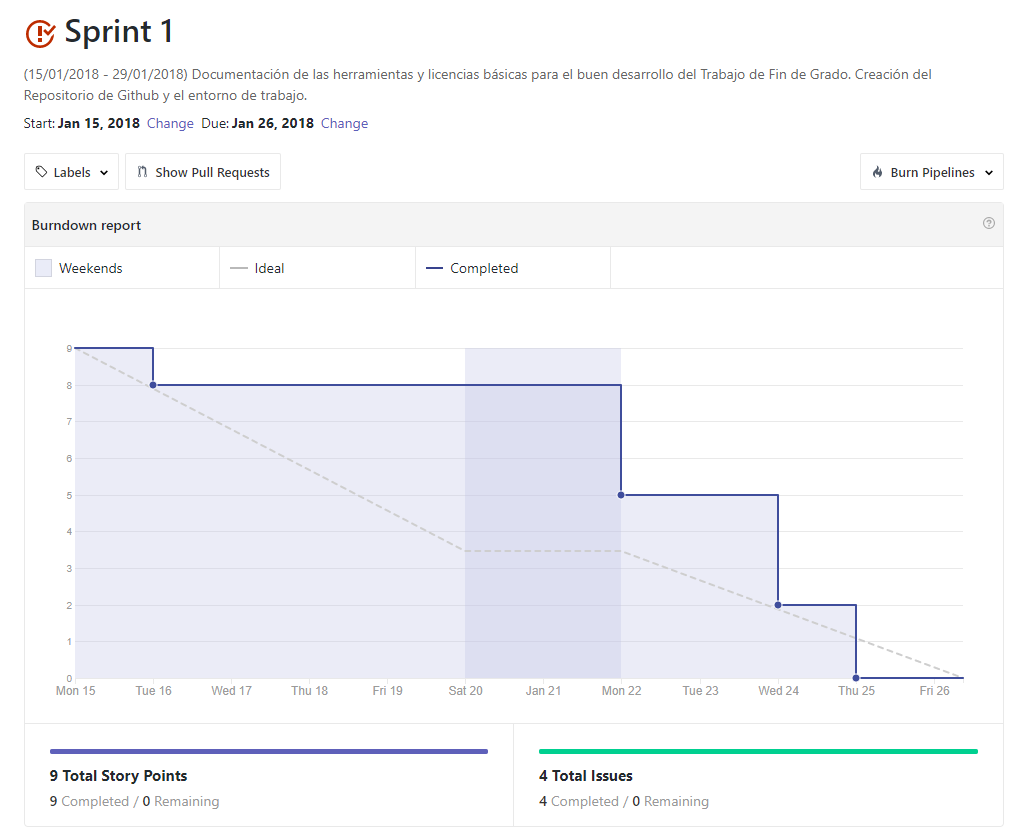
\includegraphics[width=0.90\textwidth]{Sprint_1}
\caption{Burndown del primer Sprint}
\label{fig:A.2.1}
\end{figure}

\subsection{\textbf{Sprint 2}  (29/01/2018-12/02/2018) }
El segundo Sprint, orientado hacia las técnicas utilizadas en \LaTeX así como las diferentes asígnaturas existentes en el Grado de Ingeniería Informática. Durante la reunión, se decidirá el tipo de cuestionario a realizar, y cómo orientarlo hacia la recogida de datos.  
Por ello: 
\begin{itemize}
\item Se ha comenzado el desarrollo de la Memoria en \LaTeX  y la documentación del mismo. 
\item Se han documentado las diferentes asignaturas existentes. 
\end{itemize}
\textbf{Problemáticas encontradas}\\En el segundo Sprint,hemos tenido el mismo problema que en el Sprint 1, teniendo en cuenta los ``Estimate'' como la dificultad, sin tener en cuenta que algunas tareas, a pesar de ser sencillas, tienen una mayor duración de tiempo. \\Además, nos hemos encontrado con menor tiempo, por lo que hemos tenido que traspasar un Issue al Sprint 3. \\Finalmente, hubo una confusión en el ``Due Date'', ya que habíamos considerado como el tiempo de comienzo en lugar del tiempo de fin. Dicho error fue corregido en el Sprint 3. \\La siguiente imagen corresponde al Burndown del Sprint 2~\ref{fig:A.2.2}
\begin{figure}[h]
\centering
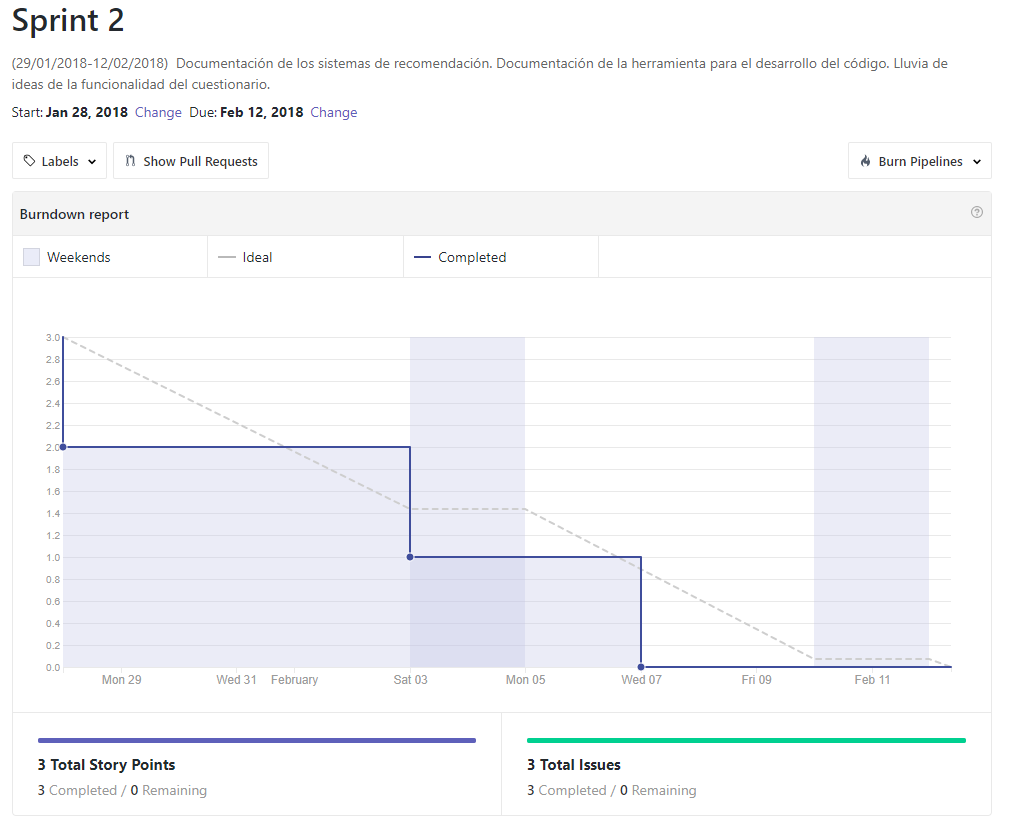
\includegraphics[width=0.90\textwidth]{Sprint_2}
\caption{Burndown del segundo Sprint}
\label{fig:A.2.2}
\end{figure}
\\

\subsection{\textbf{Sprint 3}  (13/02/2018-27/02/2018) }
El tercer Sprint, se ha orientado hacia la terminación del Sprint 2, ya que, por falta de tiempo, no se terminaron las issues. 
Por ello: 
\begin{itemize}
\item Se ha creado el formulario y distribuido entre los diferentes ex-alumnos del Grado de Ingeniería Informática en Burgos. 
\item Se ha documentado la metodología de integración de las funcionalidades del cuestionario y cómo almacenar los datos. 
\item Se ha realizado una documentación de los diferentes sistemas de Recomendación existentes.  
\end{itemize}
\textbf{Problemáticas encontradas}\\En el tercer Sprint,hemos tenido el mismo problema que en el Sprint 1 y 2, teniendo en cuenta los ``Estimate'' como la dificultad, sin tener en cuenta la duración del mismo.\\Por otro lado, al igual que en el Sprint 1 y el Sprint 2, no cerramos correctamente el Milestone, de forma que fue cerrado una vez comenzado el Sprint 4, a pesar de que las Issues se encontraban ya cerradas. \\La siguiente imagen corresponde al Burndown del Sprint 3~\ref{fig:A.2.3}
\begin{figure}[h]
\centering
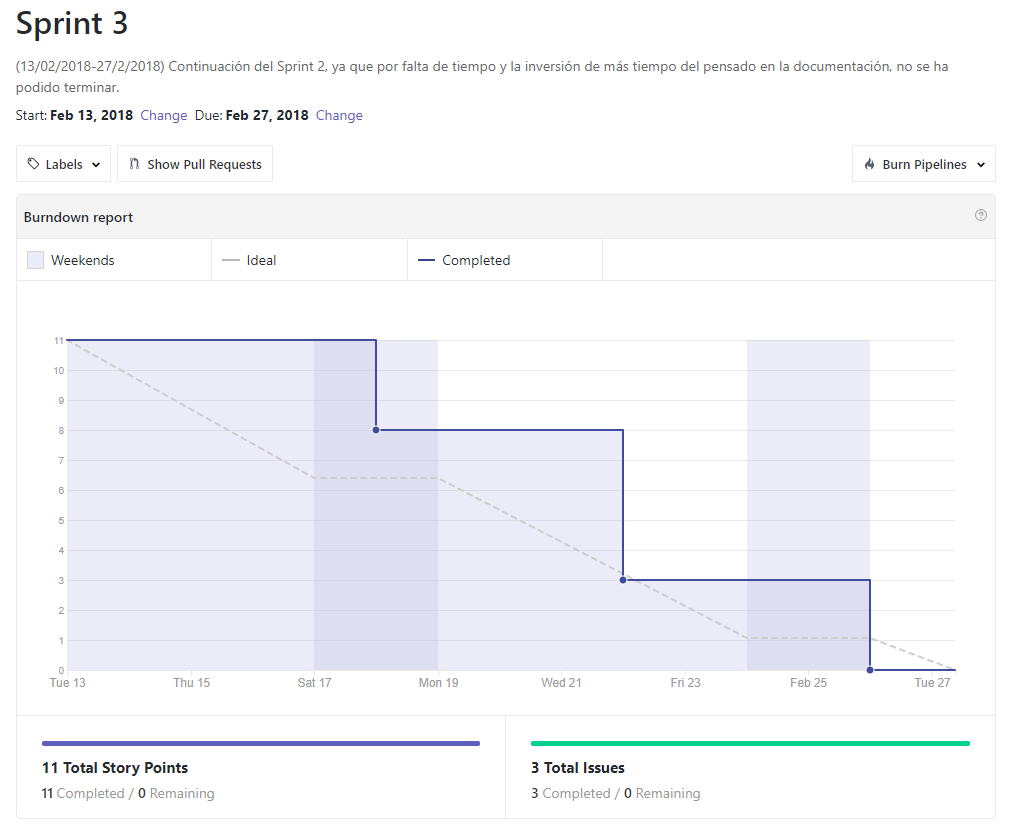
\includegraphics[width=0.90\textwidth]{Sprint_3}
\caption{Burndown del tercer Sprint}
\label{fig:A.2.3}
\end{figure}
\\

\subsection{\textbf{Sprint 4} (28/02/2018-14/03/2018) }
El cuarto  Sprint, se ha orientado hacia la integración de los resultados del cuestionario anónimo en Python, así como el desarrollo y corrección de memorias y anexos. 
Por ello: 
\begin{itemize}
\item Se han corregido las memorias y anexos, centrándonos en los errores ortográficos existentes.  
\item Se han creado las tablas explicativas de las memorias y anexos. 
\item Se ha documentado acerca de la API existente para sincronizar de forma dinámica los datos de Google Drive sin necesidad de descargar el fichero Excel. Para ello, se ha escogido la herramienta API GOOGLE-DIVE. 
\item Se ha desarrollado el código de integración de los datos-recogidos en el cuestionario- en Python.   
\end{itemize}
\textbf{Problemáticas encontradas}\\En el cuarto Sprint,tras sincronizar los datos del Excel con la API, y descargar el fichero json, hemos visto que los datos en Python no se sincronizan automáticamente, sino que se debe sincronizar manualmente de forma previa a la ejecución del código. Sin embargo, al ser el Admin quien se encarga de dicha tarea, no se considera un problema incompatible con la idea inicial del proyecto.  
 \\La siguiente imagen corresponde al Burndown del Sprint 4~\ref{fig:A.2.4}
\begin{figure}[h]
\centering
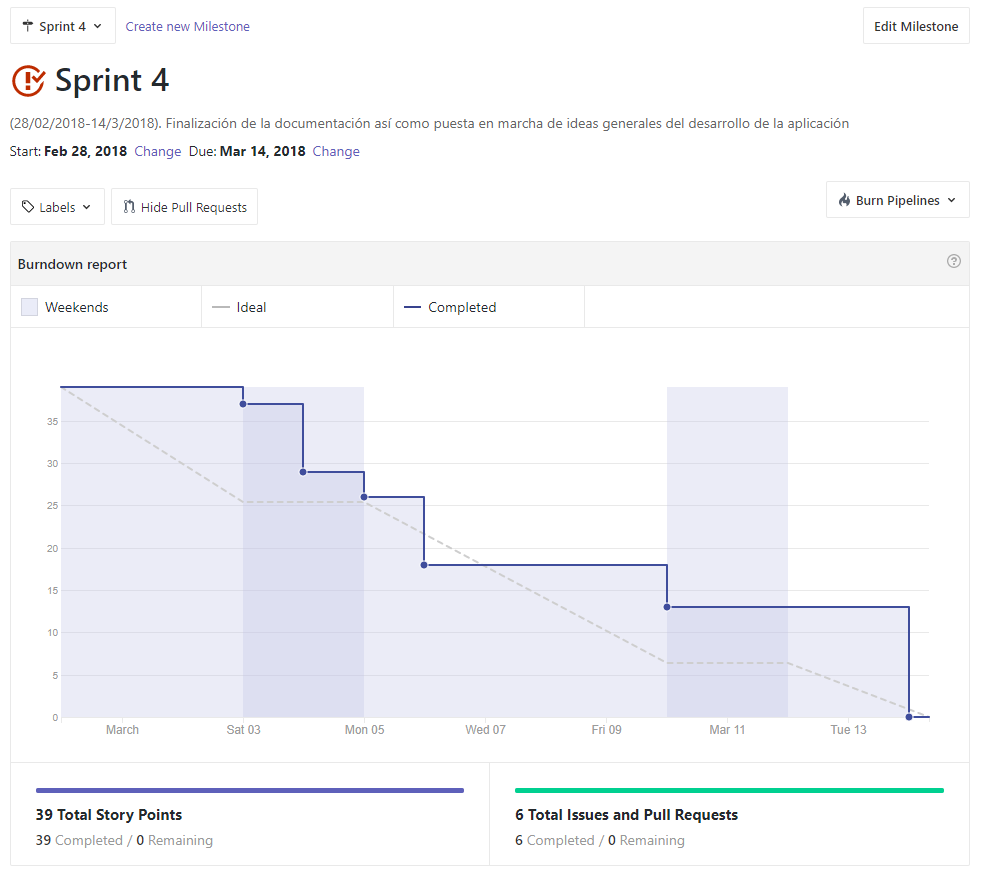
\includegraphics[width=0.90\textwidth]{Sprint_4}
\caption{Burndown del cuarto Sprint}
\label{fig:A.2.4}
\end{figure}
\\

\subsection{\textbf{Sprint 5} (15/03/2018-28/03/2018) }
El quinto  Sprint, se ha orientado hacia la documentación y el desarrollo del sistema de recomendación basado en productos. 
Por ello: 
\begin{itemize}
\item Se ha documentado el modo de diseño de la interfaz gráfica y probado su funcionamiento.   
\item Se ha desarrollado el sistema de recomendación basado en productos.  
\item Se ha desarrollado el plan de proyecto del Sprint 4.
 
\end{itemize}
\textbf{Problemáticas encontradas}\\En el quinto Sprint,nos hemos encontrado con la problemática de la dificultad del desarrollo del sistema de recomendación basado en productos de forma que no fuese necesario repetir diferentes funciones, simplificándolo, de forma que los métodos sean compatibles tanto  para el sistema de recomendación basado en usuarios como con el sistema de recomendación basado en productos. 
 \\La siguiente imagen corresponde al Burndown del Sprint 5~\ref{fig:A.2.5}
\begin{figure}[h]
\centering
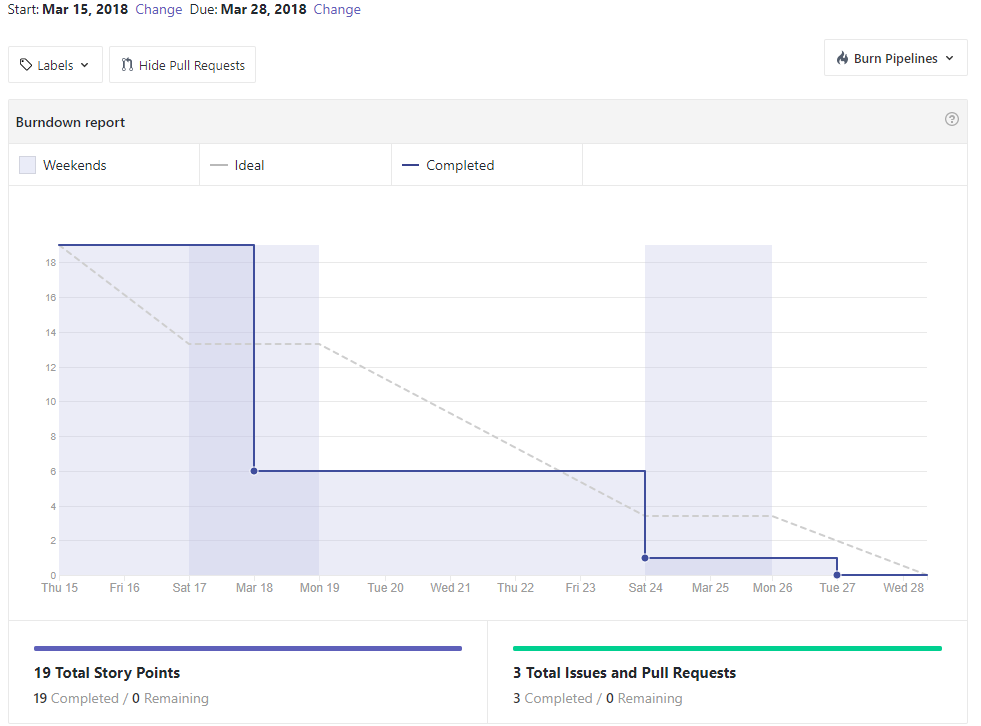
\includegraphics[width=0.90\textwidth]{Sprint_5}
\caption{Burndown del quinto Sprint}
\label{fig:A.2.5}
\end{figure}
\\

\subsection{\textbf{Sprint 6} (29/03/2018-12/04/2018) }
El sexto  Sprint, se ha orientado hacia la documentación, el desarrollo  y corrección de  diferentes sistemas de recomendación, así como la documentación del modo de almacenamiento de la información de los usuarios y asignaturas en cloud.  
Por ello: 
\begin{itemize}
\item Se ha documentado del sistema de recomendación basado en modeloSe ha documentado del modo de almacenamiento de los datos de los usuarios en cloud. 
\item Se ha continuado con el desarrollo de memorias y anexos. 
\item Se ha corregido el sistema de recomendación basado en productos. 
\item Se ha desarrollado el código del sistema de recomendación basado en usuarios.  

\end{itemize}
\textbf{Problemáticas encontradas}\\En el sexto Sprint,nos hemos encontrado con la problemática de cómo poder almacenar los datos de los usuarios de forma que se pudiese validar el usuario y contraseña, con un API que fuese gratuito. Por otra parte, hemos observado que hay un límite de llamadas al API que accede a  los datos almacenados en Google Drive. Esto no es un impedimento en el acceso a los mismos, ya que, al almacenar los datos en un fichero binario tras la carga, no es necesario realizar la llamada en cada ejecución del sistema de recomendación. 
 \\La siguiente imagen corresponde al Burndown del Sprint 6~\ref{fig:A.2.6}
\begin{figure}[h]
\centering
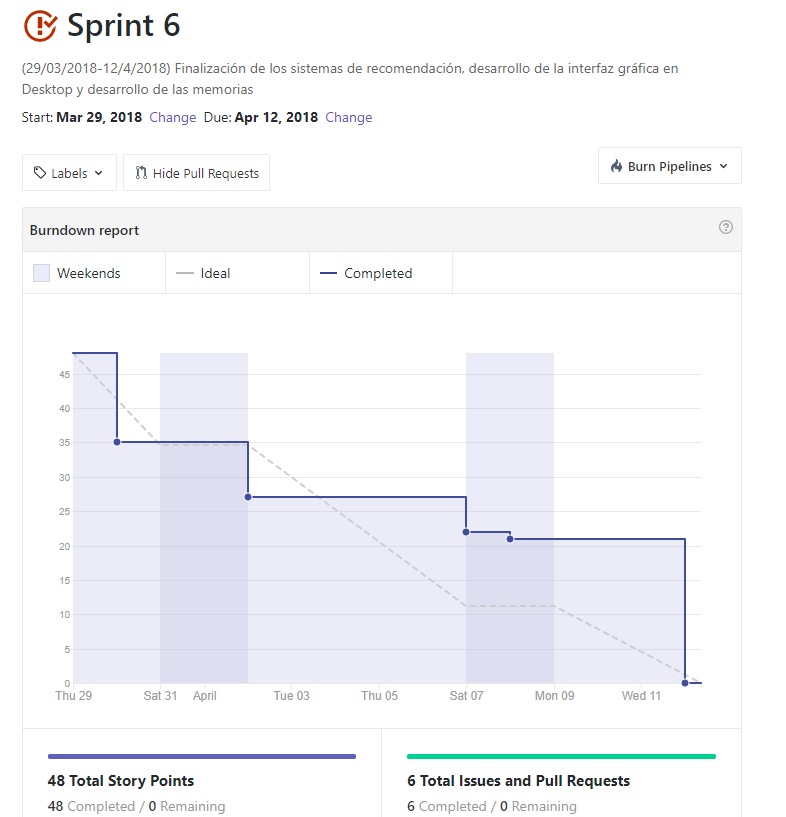
\includegraphics[width=0.90\textwidth]{Sprint_6}
\caption{Burndown del sexto Sprint}
\label{fig:A.2.6}
\end{figure}
\\



\subsection{\textbf{Sprint 7} (13/04/2018-27/04/2018) }
El séptimo  Sprint, se ha orientado hacia la documentación y  el desarrollo de memorias y anexos, así como la adaptación de los notebooks para ser utilizados en Eclipse utilizando el IDE de Python, PyDev. 
Por ello: 
\begin{itemize}
\item Se ha decidido la herramienta de desarrollo del proyecto. 
\item Se ha continuado con el desarrollo de memorias y anexos. 
\item Se ha desarrollado el plan de proyecto del Sprint 6.
\item Se ha adaptado el código de los notebooks en diferentes clases. 

\end{itemize}
\textbf{Problemáticas encontradas}\\En el Sprint 7, se continuó el desarrollo del sistema de recomendación basado en modelo, sin embargo, habiendo finalizado el Sprint, no se terminó con el código, por lo que se transpasó al  siguiente Sprint. 
 \\La siguiente imagen corresponde al Burndown del Sprint 7~\ref{fig:A.2.7}
\begin{figure}[h]
\centering
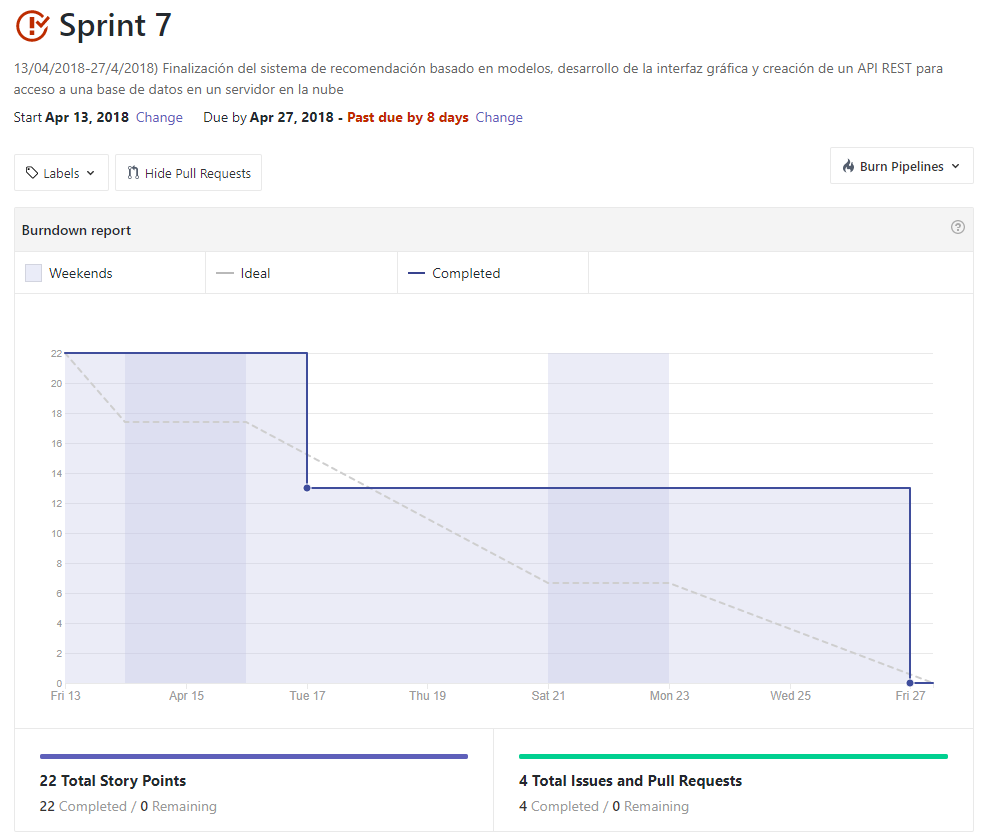
\includegraphics[width=0.90\textwidth]{Sprint_7}
\caption{Burndown del séptimo Sprint}
\label{fig:A.2.7}
\end{figure}
\\

\subsection{\textbf{Sprint 8} (28/04/2018-12/05/2018) }
El octavo  Sprint, se ha orientado hacia el desarrollo de memorias y anexos, tablas explicativas de las asignaturas para el desarrollo de posteriores gráficas, así como el desarrollo del sistema de recomendación basado en modelos. 
Por ello: 
\begin{itemize}
\item Se ha desarrollado el código del sistema de recomendación basado en modelos. 
\item Se ha continuado con el desarrollo de memorias y anexos. 
\item Se ha desarrollado el plan de proyecto del Sprint 7.
\item Se han creado las Entity necesarias (Usuarios  y Asignatura). 
\item Se ha creado en Excel la tabla explicativa del contenido general de las asignaturas. 
\end{itemize}
\textbf{Problemáticas encontradas}\\En el Sprint 8, se comenzó el desarrollo de los Requisitos Funcionales, a pesar de no haberse podido terminar, así como la adaptación a \LaTeX de la misma. Por otro lado, se comenzó el diseño de una posible interfaz gráfica versión 1.0, no habiéndose finalizado. \\Otra problemática encontrada ha sido un bug en el código del sistema de recomendación basado en modelos que aun no ha sido corregido. 
 \\La siguiente imagen corresponde al Burndown del Sprint 8~\ref{fig:A.2.8}
\begin{figure}[h]
\centering
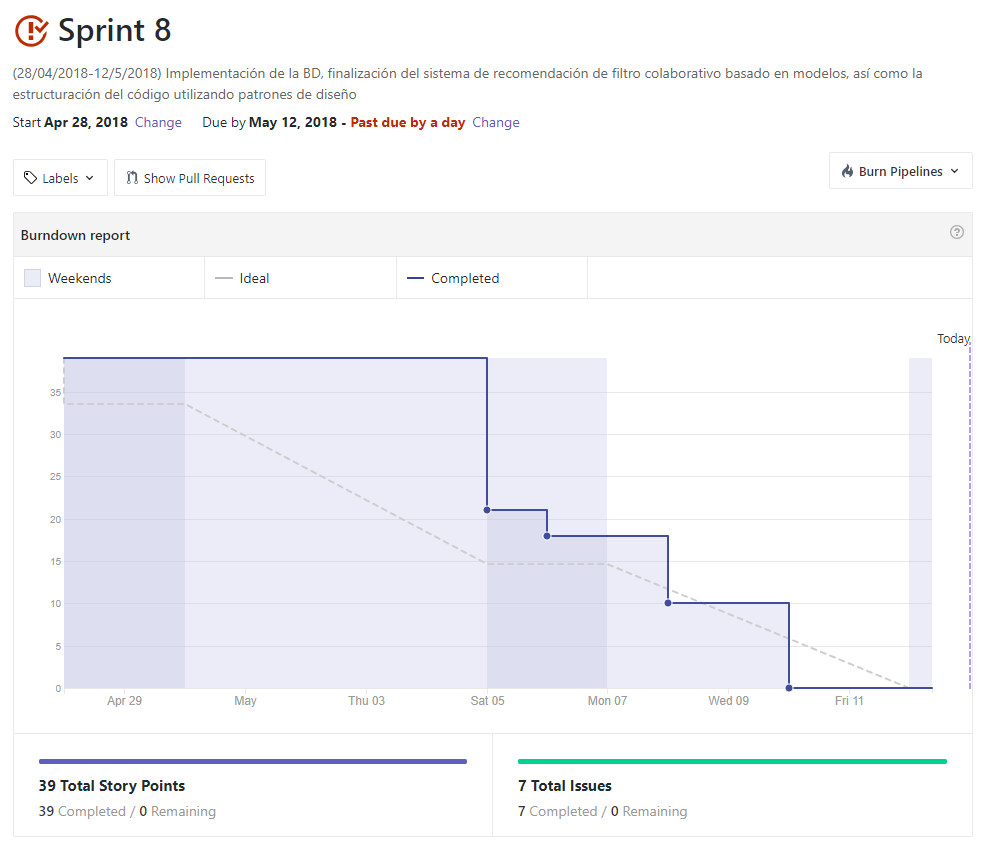
\includegraphics[width=0.90\textwidth]{Sprint_8}
\caption{Burndown del octavo Sprint}
\label{fig:A.2.8}
\end{figure}
\\

\subsection{\textbf{Sprint 9} (13/05/2018-27/05/2018) }
El noveno  Sprint, se ha orientado hacia el desarrollo de memorias y anexos, el diseño de la estructura de clases y paquetes tanto del Core como de la interfaz gráfica, el desarrollo del código de la interfaz gráfica, así como la autenticación del usuario en la BD y la reestructuración del código. 
Por ello: 
\begin{itemize}
\item Se ha realizado un diseño de posible gráfica para desarrollar. 
\item Se han corregido memorias y anexos.
\item Se ha desarrollado el plan de proyecto del Sprint 8.
\item Se ha desarrollado el manual de usuario.
\item Se han creado los diagramas de clases del Core y de la GUI. 
\item Se ha adaptado el código del sistema de recomendación basado en usuarios y modelos para la simplificación del mismo. 
\item Se ha desarrollado el apéndice Diseño. 
\item Se ha desarrollado la primera y segunda pestaña de la interfaz. 
\end{itemize}
\textbf{Problemáticas encontradas}\\En el Sprint 9, se ha tenido un problema con la subida del paquete src del proyecto, por lo que se tuvo que  volver a subir el código del Workespace con el que se estaba trabajando. Por otra parte, no se ha solucionado el  bug del sistema de recomendación basado en modelos, por lo que se ha dejado dicha pestaña bloqueada. 
 \\La siguiente imagen corresponde al Burndown del Sprint 9~\ref{fig:A.2.9}
\begin{figure}[h]
\centering
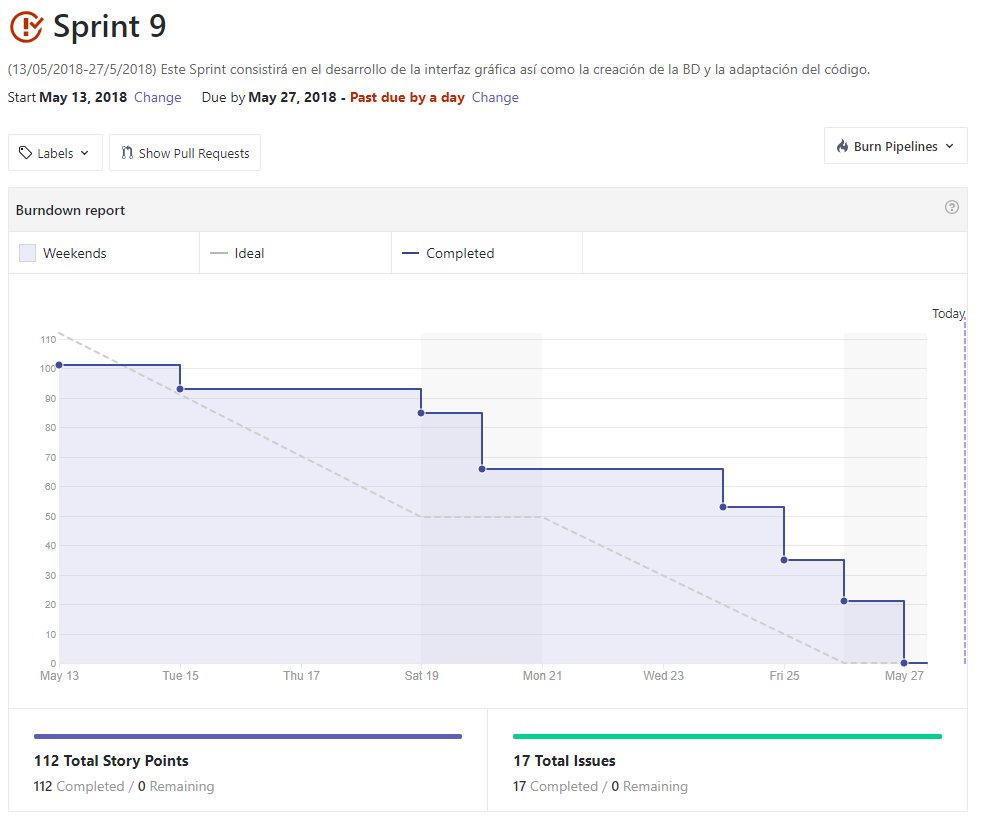
\includegraphics[width=0.90\textwidth]{Sprint_9}
\caption{Burndown del noveno Sprint}
\label{fig:A.2.9}
\end{figure}
\\

\apendice{Especificación de Requisitos}
Este apéndice se subdivide en los diferentes requisitos necesarios para nuestro proyecto, en su realización y subdivisión. 
\section{Objetivos Generales}
\begin{enumerate}
\item Construcción de un cuestionario anónimo para la recogida de datos iniciales para ser utilizados en el entrenamiento de los sistemas de recomendación. 
\item Desarrollo de diferentes sistemas de recomendación, su entrenamiento en base a los datos recogidos y la devolución de las ponderaciones de las asignaturas no cursadas por un usuario. 
\item Desarrollo de una interfaz gráfica modo usuario para una mejor utilización de los mismos, de forma que las recomendaciones mostradas por el sistema de recomendación sean específicas para determinado usuario. 
\item Desarrollo de una interfaz gráfica modo administrador para la modificación, agregación o eliminación de diferentes calificaciones. 
\end{enumerate}
\section{Catálogo de Requisitos}
\begin{itemize}
\item RF-1. Recogida de datos\\ 
\begin{itemize}
\item RF-1.1. Creación de cuestionario anónimo.\\ 
\item RF-1.2. Distribución del cuestionario. \\ 
\item RF-1.3. Recogida de datos y su almacenamiento. 
\end{itemize}

\item RF-2. Desarrollo de los sistemas de recomendación\\ 
\begin{itemize}
\item RF-2.1. Recogida de datos de Drive. 
\item RF-2.2. Tratamiento de los datos. 
\item RF-2.3. Desarrollo del sistema de recomendación. 
\item RF-2.4. Devolución de las calificaciones. \item Guardado de los datos. 
\end{itemize}

\item Desarrollo de una interfaz gráfica \\ \begin{itemize}
\item Construcción de pestaña de inicio sesión.  \item Lectura de datos almacenados. \item Obtención de datos del registro de usuario. \item Generación de recomendación de calificaciones. \item Muestra de gráficos de calificaciones en diferentes asignaturas. \item Acceso a los datos generales en modo administrador. 
\end{itemize}
\end{itemize}

\section{Especificación de Requisitos}
\begin{itemize}
\item Construcción de ventana de inicio de sesión. 
\begin{itemize}
\item Construcción de botón de inicio sesión. 
\item Construcción de áreas para rellenar usuario y contraseña.  
\item Construcción de la funcionalidad para acceder a la Base de Datos. 
\item Construcción de la funcionalidad para validar usuario y contraseña. 
\end{itemize}
\item Construcción de la pestaña inicial para rellenar el cuestionario para ponderar las asignaturas cursadas. 
\begin{itemize}
\item Construcción del botón de selección del Sistema de Recomendación.
\item Construcción de funcionalidad para llamar al sistema de recomendación  seleccionado. 
\item Construcción de la funcionalidad para ejecutar el sistema de recomendación con los datos rellenados. 
\item Construcción de la funcionalidad para mostrar las calificaciones resultantes no cursadas. 
\end{itemize}
\item Construcción de la funcionalidad del guardado y  el tratamiento de los datos. 
\begin{itemize}
\item Construcción de la funcionalidad de recogida de datos de Drive. 
\item Construcción de la funcionalidad del tratamiento de los datos recogidos. 
\item Construcción de la funcionalidad para el guardado de los datos. 
\end{itemize}
\end{itemize}

\section{Diagramas de Casos de Uso}
\subsection{Diagrama General}
El siguiente diagrama corresponde al  caso de uso general, junto con el diagrama extendido. \ref{fig:Diagrama_Caso_Uso_General}
\begin{figure}[h]
\centering
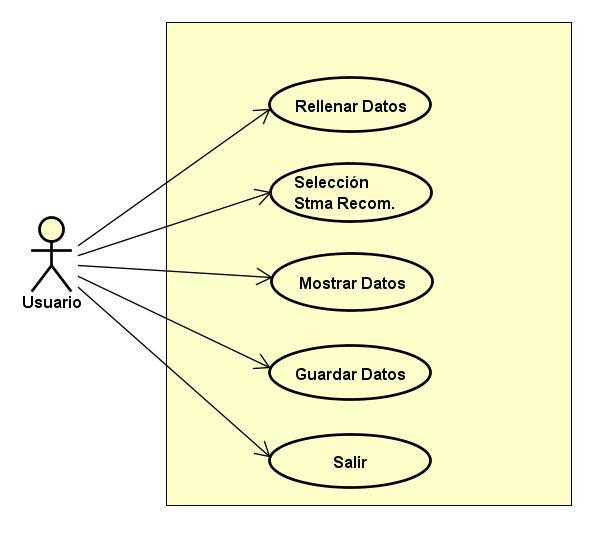
\includegraphics[width=0.90\textwidth]{Diagrama_Caso_Uso_General}
\caption{Diagrama de caso de uso General}
\label{fig:Diagrama_Caso_Uso_General}
\end{figure}

\section{Tablas de Casos de Uso}
\subsection{Primer Caso de Uso}
La primera tabla corresponde al desarrollo del cuestionario anónimo y la recogida de datos para poder trabajar posteriormente con ellos. La siguiente tabla hace referencia al dicho caso de uso. \ref{tab:1}
\begin{table}[]
\caption{Tabla Caso de Uso 1}
\label{tab:1}
\resizebox{\textwidth}{!}{
\begin{tabular}{ lrrr }
\toprule
\textbf{Nombre} &   Recogida de Datos         \\ 
\textbf{Versión} & 1.0  \\ 
\textbf{Requisitos Funcionales}  & \begin{tabular}[c]{@{}l@{}}RF-1\\ RF-1.1\\ RF-1.2\\ RF-1.3\\\end{tabular}                                                                                                                  \\ 
\textbf{Descripcíon de Requisitos} & \begin{tabular}[r]{@{}l@{}}Se obtendrán los datos de forma anónima  para el entrenamiento\\ de los sistemas de recomendación\\\end{tabular}                                                                                                                    \\
\textbf{Precondiciones}     & No tiene \\
\textbf{Postcondiciones}         &  Se almacenarán los datos en una API de Google \\
\textbf{Autor}         & Clara Palacios Rodrigo \\
\textbf{Importancia}        &  Importante \\ \bottomrule
\end{tabular}
}
\end{table}

\subsection{Segundo Caso de Uso}
La segunda tabla corresponde con el desarrollo de los sistemas de recomendación. Para ello, se debe obtener los datos de la API de Drive, tratarlos y desarrollar los diferentes sistemas de recomendación. La siguieten tabla hace referencia a dicho caso de uso. \ref{tab:2}
\begin{table}[]
\caption{Tabla Caso de Uso 2}
\label{tab:2}
\resizebox{\textwidth}{!}{
\begin{tabular}{ lrrr }
\toprule
\textbf{Nombre} &   Desarrollo de los sistemas de recomendación        \\ 
\textbf{Versión} & 1.0  \\ 
\textbf{Requisitos Funcionales}  & \begin{tabular}[c]{@{}l@{}}RF-2\\ RF-2.1\\ RF-2.2\\ RF-2.3\\RF-2.4\end{tabular}                                                                                                                  \\ 
\textbf{Descripcíon de Requisitos} &  \\
\textbf{Precondiciones}     & Disponer de los datos en Drive \\
\textbf{Postcondiciones}         &   \\
\textbf{Autor}         & Clara Palacios Rodrigo \\
\textbf{Importancia}        & Muy Importante \\ \bottomrule
\end{tabular}
}
\end{table}




\apendice{Especificación de diseño}

\apendice{Documentación técnica de programación}
En este apéndice, incluiremos las bases de programación y desarrollo del proyecto necesarias para un buen funcionamiento del Sistema de Recomendación. 

\section{Recogida de datos}
La recogida de datos se desarrolla utilizando un cuestionario anónimo en web, utilizando la página Typeform, de forma que se deben introducir de forma obligatoria las calificaciones de los tres primeros cursos. En este proyecto, hasta la fecha, 56 alumnos y ex-alumnos han rellenado dicho cuestionario. 
\subsection{Creación del cuestionario}
El cuestionario se ha creado utilizando la página gratuita de Typeform, modificando el aspecto del cuestionario y añadiendo las asignaturas y sus restricciones. 
Se procedió al  guardado de los ficheros en un documento Excel en Google Drive, denominado "DatosTFG\_SistemasRecomendacion". 

\subsection{Obtención de los datos}
Para obtener los datos almacenados en Drive, se ha necesitado activar el API GoogleDrive, para poder acceder a los datos sin necesidad de descargar continuamente el fichero. Para ello: 
\begin{itemize}
 
\item Acceder a \url{https://console.developers.google.com/apis/library}
\item Crear un nuevo proyecto\ref{fig:D.1.1}. Se debe tener en cuenta que hay un número máximo de proyectos creados de forma gratuita.
\begin{figure}[h]
\centering
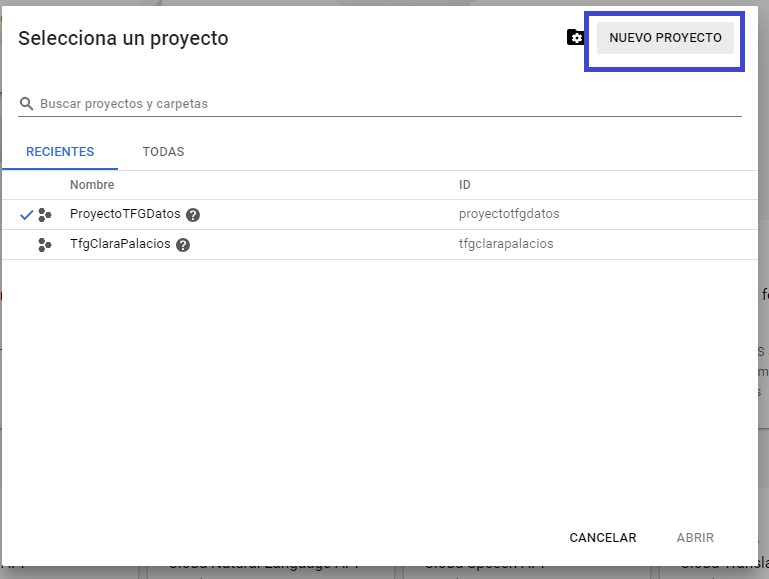
\includegraphics[width=0.90\textwidth]{crear_proyecto_api}
\caption{Crear proyecto nuevo}
\label{fig:D.1.1}
\end{figure}  
\item Introducir el nombre del proyecto creado y pulsar Crear.\ref{fig:D.1.2} 
\begin{figure}[h]
\centering
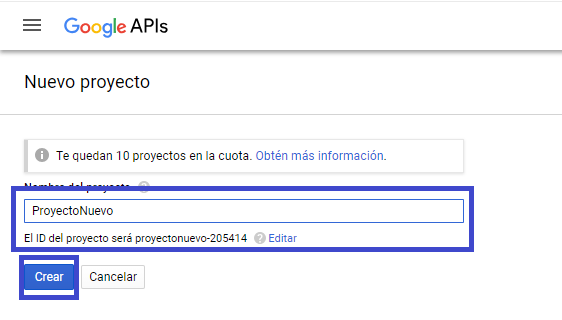
\includegraphics[width=0.90\textwidth]{nombre_proyecto_api}
\caption{Dar nombre al proyecto}
\label{fig:D.1.2}
\end{figure}  
\item Acceder a \url{https://console.developers.google.com/}
\item Buscar GoogleDrive API, y activar dicha API.\ref{fig:D.1.3} 
\begin{figure}[h]
\centering
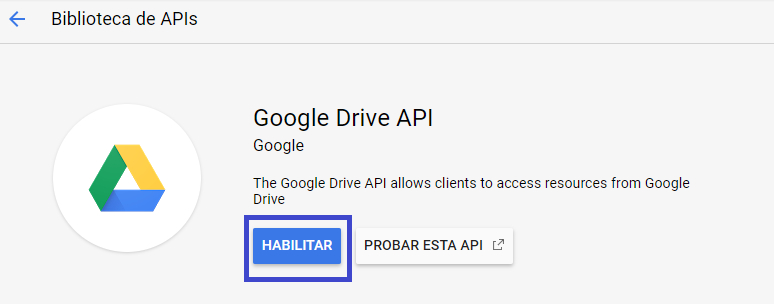
\includegraphics[width=0.90\textwidth]{activar_google_drive}
\caption{Activar Google Drive}
\label{fig:D.1.3}
\end{figure}  
\item Activar credenciales para el proyecto creado\ref{fig:D.1.3} 
\begin{figure}[h]
\centering
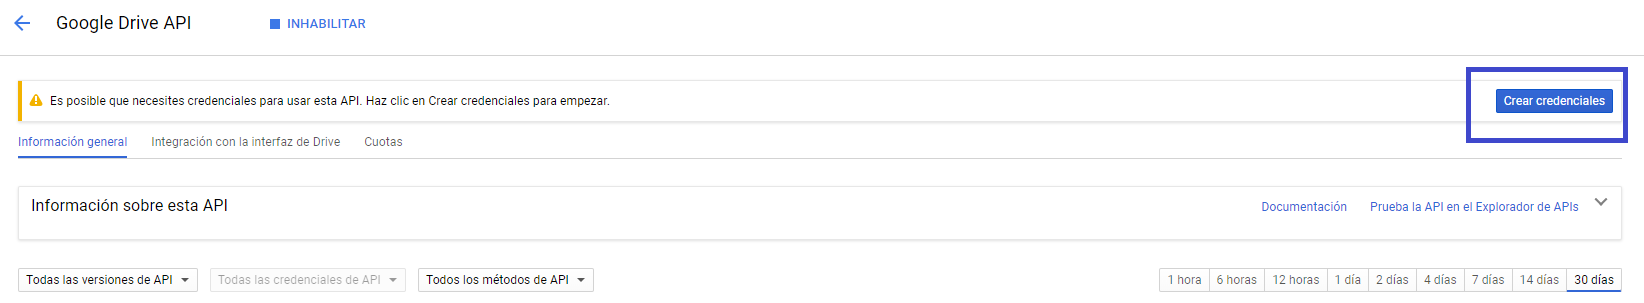
\includegraphics[width=0.90\textwidth]{credenciales_proyecto_api}
\caption{Obtener Credenciales}
\label{fig:D.1.3}
\end{figure}  
\item Activar las credenciales para acceder al documento en Google Drive. \ref{fig:D.1.4} De esta forma, un cliente puede acceder a dichos datos. (El administrador en este caso). Pulsar ``Qué credenciales necesito''
\begin{figure}[h]
\centering
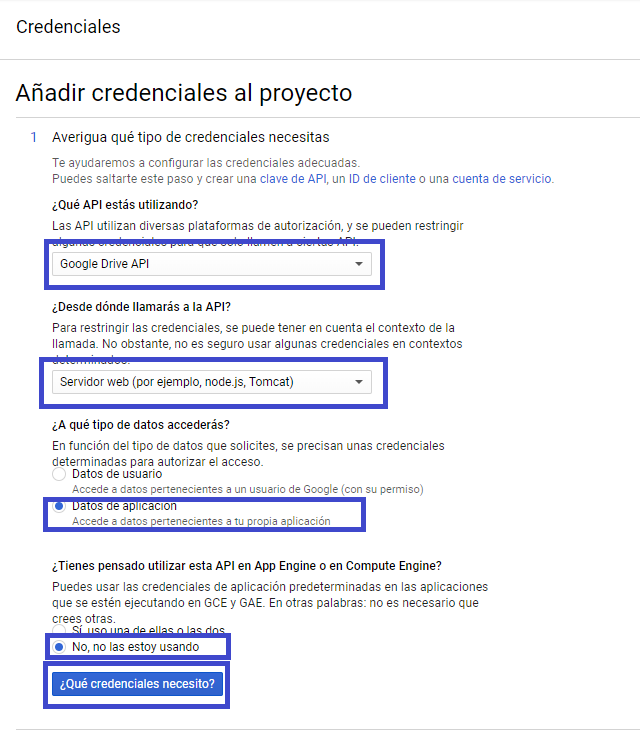
\includegraphics[width=0.90\textwidth]{credenciales_seleccionar_api}
\caption{Activar Credenciales}
\label{fig:D.1.4}
\end{figure}  
\item Introducir el rol que se le dará, así como el nombre del servicio. \ref{fig:D.1.5}
\begin{figure}[h]
\centering
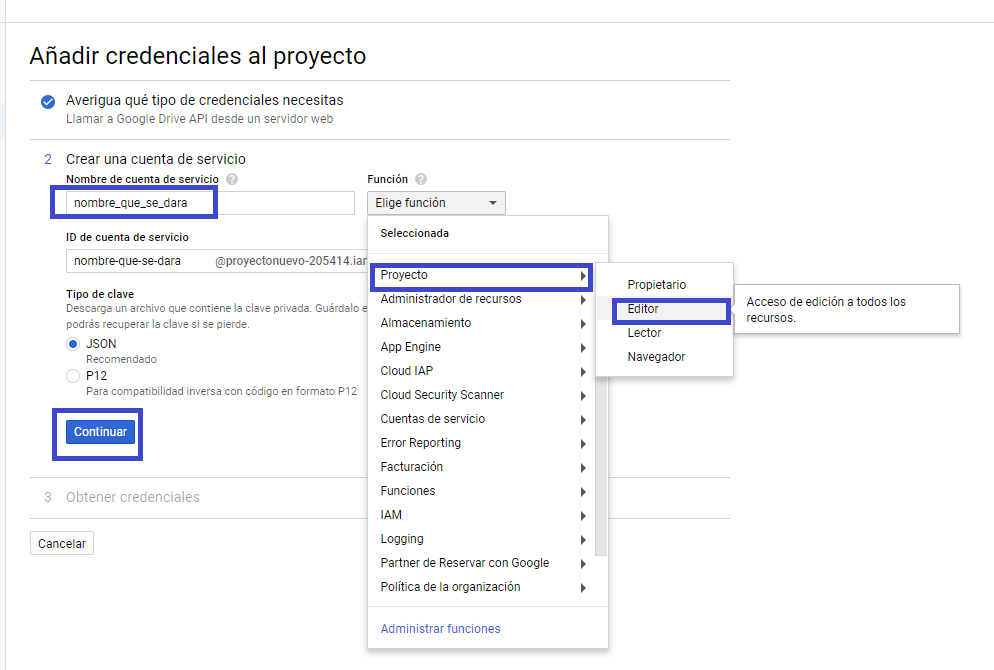
\includegraphics[width=0.90\textwidth]{nombre_rol_api}
\caption{Introducir nombre y rol}
\label{fig:D.1.5}
\end{figure}
\item Tras pulsar continuar, se descargará un fichero json, y mostrará un mensaje por pantalla. 
\item Abrir el fichero json y copiar el correo electrónico obtenido, compartiéndolo en el documento existente en Google Drive. 
\end{itemize}
Una vez pudiendo acceder a dichos datos, se debe acceder desde el código utilizando la librería ServiceAccountCredentials. Se debe tener en cuenta que el fichero json debe de encontrarse en el mismo directorio que el código que desee acceder al mismo. 


\section{Tratamiento de los datos}
Los datos recibidos desde la API contienen columnas no necesarias para el proyecto, tales como el Token y la fecha de rellenado. Por otra parte, al recibir los datos, en caso de no haberse cursado, el valor será un string vacío, por lo que habrá que modificar ese string por un NaN (de la librería numpy), para diferenciar de las calificaciones marcadas con cero por los usuarios.   Los datos devueltos por esta función de tratamiento se almacenan en un dataframe.

\section{Sistemas de recomendación}
El desarrollo de los sistemas de recomendación se simplifica reutilizando las funciones de cálculo de matriz de similitud y de matriz de distancias, realizándolas de forma genérica para evitar la duplicidad del código. 
\subsection{Basado en usuarios y productos}
Se recibe la matriz de similitud y el diccionario de las asignaturas del cuarto curso para calcular la predicción de las asignaturas y devolvérselas. 

\subsection{Util}
El paquete util implementa tanto el coeficiente de Pearson como la matriz de similitud. 
\subsubsection{Distancias}
Par el cálculo del coeficiente de pearson se recibe el dataframe junto con las variables a y b, que en uno de los filtros colaborativos son usuarios mientras que en el otro son items. De esta forma, el código puede ser reutilizado para ambos sistemas de recomendación. 
\subsubsection{Matriz\_Similitud}
En la misma línea, el cálculo de la matriz de similitud se realiza de forma genérica para poder acceder tanto por el filtro colaborativo basado en usuarios como por el filtro colaborativo basado en productos. Esta clase recibe el dataframe de los datos con los que se trabajará, calcula la matriz de similitud con todos los elementos y devuelve una matriz de similitud elemento-elemento. 

\section{I\_O\_Datos}
El paquete I\_O\_Datos implementa la recuperación de datos tanto de drive, de un fichero binario o de la base de datos. De esta forma:
\subsection{Binario}
Para la lectura de datos en binario, se obtiene todo el dataframe eliminándose las columnas innecesarias,  y devolviéndose un dataframe con el que se pueda trabajar. 

\subsection{GoogleDrive}
El funcionamiento de esta opción se ha realizado en la primera sección de forma que no se entrará en detalles.

\subsection{API\_Rest}
En esta clase, se obtienen-a través de un json- y se almacenan los datos de Cloud reemplazando tildes y espacios en blanco de los nombres de las asignaturas. Por otra parte, se deben eliminar las columnas no necesarias. 
Finalmente, la clase devuelve un dataframe para poder trabajar con él. 

\section{Diccionario}
El diccionario utilizado sirve tanto para los elementos de la interfaz gráfica (secciones, botones...) como el almacenamiento y subdivisión de las asignaturas por semestres, así como la caracterización de las mismas. 

\section{Interfaz gráfica}
La interfaz gráfica se ha desarrollado utilizando PyQt5. Para su estructura, se ha subdividido el código en paquetes, de forma haya un paquete por cada pestaña y un panel de pestañas y la ventana principal. 
\subsection{Asignaturas}
Este paquete contienen las asignaturas de cada curso para la primera pestaña, junto con los layout y checkbox para modificar sus ponderaciones. Por otra parte, la clase ``Asignatura'' Implementa los métodos de guardado de los datos y carga de los mismos. 

\subsection{Modelos}
Este paquete implementa las clases para la muestra de los resultados de las asignaturas, así como las gráficas relacionadas con dichos resultados. Esto está implementado en la clase TopCuartoFrame, clase encargada de pintar los resultados. \\Para su obtención, desde la clase Modelos del mismo paquete se implementan las funciones para ejecutar los filtros colaborativos y establecer las asignaturas del curso que vayan a aparecer en la pestaña. 

\subsection{Estadísticas}
Corresponde con la tercera pestaña de gráficos auxiliares para el usuario. Este paquete contiene los cuatro cursos para mostrar sus nombres en el área de las leyendas y su media, mediana, máximo y mínimo en las gráficas. Estos cálculos se realizan en el paquete estadística, así como el establecimiento de las barras verticales correspondientes a las asignaturas.


\section{Base de Datos} 
El procedimiento para almacenar los usuarios y ponderaciones, así como los datos de entrenamiento para los sistemas de recomendación, en la base de datos es uno de los temas más importantes de este proyecto, por lo que consideramos conveniente introducir una sección expresamente para desarrollarlo. 
El acceso directo a la base de datos en Cloud no es viable en nuestro caso, no podemos acceder a los datos en sí, sino a los End Points, ya que el acceso a la Base de Datos no es gratuita, por lo que se debería de utilizar un API de forma intermedia que acceda a dichos datos. 
El API que accede a la BD debe estar alojado directamente en el mismo lugar del Host de PythonAnyWhere. 
\subsection{Swagger}
Swagger es una herramienta elegida para consumir APIs REST. Nosotros utilizaremos dicha herramienta para validar los usuarios y contraseñas, así como para registrarse, eliminar un usuario o modificarlo. 
La dirección del swagger utilizada es la siguiente:  \url{http://claratfg2.pythonanywhere.com/apidocs/}
\\Para obtener todos los usurios, basta con ejecutar la función User\_Get\_All del swagger, dándonos todos los usuarios existentes que se hayan registrado,  con sus contraseñas encriptadas. Al pulsar Try-out, se ejecuta la función correspondiente. Un ejemplo de la obtención de todos los usuarios es la siguiente: \ref{fig:D.1.6}
\begin{figure}[h]
\centering
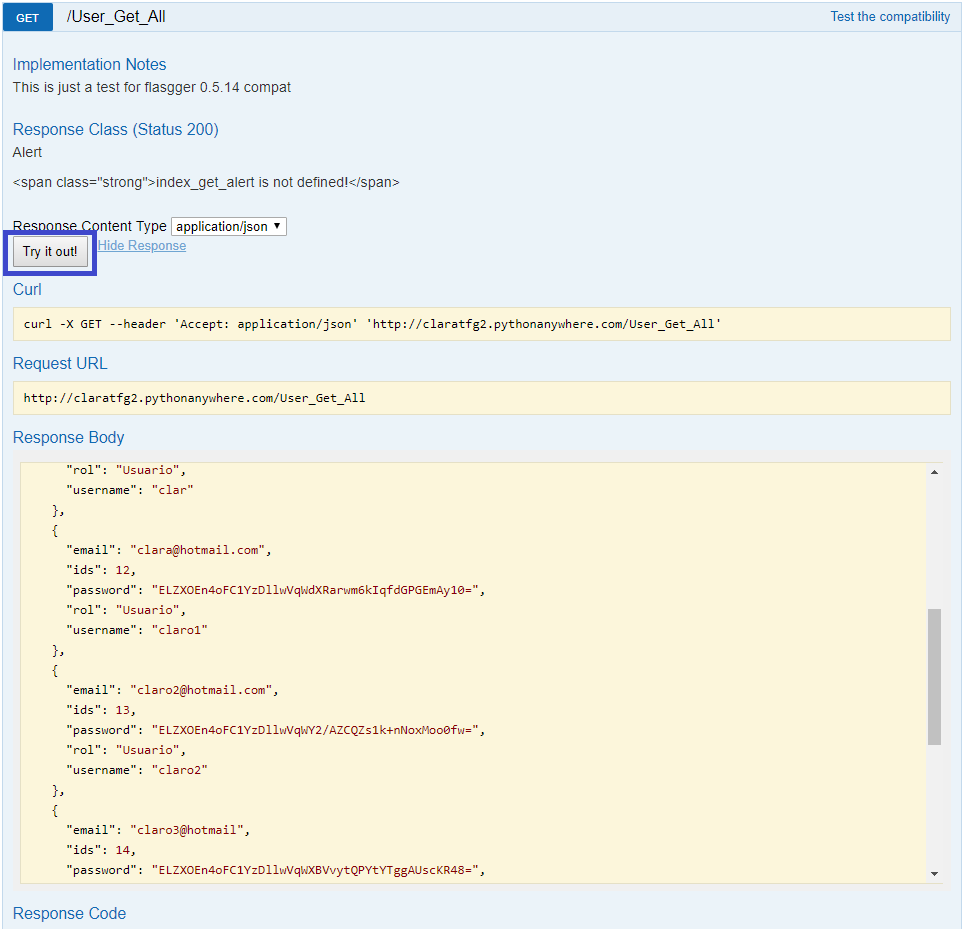
\includegraphics[width=0.90\textwidth]{swagger}
\caption{Obtención de los usuarios, swagger}
\label{fig:D.1.6}
\end{figure}
\\Para evitar que cualquier usuario acceda al swagger se podría implementar una contraseña para el acceso. Sin embargo, por falta de tiempo, recursos y conocimientos no se ha realizado dicha implementación. 

\apendice{Documentación técnica de Usuario }

\section{Requisitos previos}
\subsection{Modo usuario}
De forma previa a la utilización de la aplicación, se deberá tener instalado en el equipo lo siguiente: 
\begin{itemize}
\item \textbf{Sistema operativo}
\begin{itemize}
\item Windows
\end{itemize} 
\item \textbf{Distribución}
\begin{itemize}
\item Anaconda en su última versión estable 5.6, con la versión de Python 3.6. Dicha descarga se puede realizar a través del siguiente enlace: \url{https://www.anaconda.com/download/}
\end{itemize}
\item \textbf{Librerías  y Paquetes auxiliares}
\begin{itemize}
\item Matplotlib en la versión 2.0 o superior. En caso de no disponer de dicha librería actualizada, se puede actualizar con el siguiente comando: "conda update --all".
\item flask con el comando "pip install flask"
\item flask\_marshmallow con el comando "pip install flask\_marshmallow"
\item flasgger con el comando "pip install flasgger"
\item SQLAlchemy con el comando "pip install SQLAlchemy" y el comando "pip install flask\_sqlalchemy"
\end{itemize}
\item \textbf{Proyecto}
\begin{itemize}
\item Descargar o clonar el proyecto TFG-Sistema\_de\_recomendacion\_Asignaturas\_Optativas a través del siguiente enlace: \url{https://github.com/ClaraPalacios/TFG-Sistema_de_recomendacion_Asignaturas_Optativas/issues}
\end{itemize}
\item \textbf{Otros}
\begin{itemize}
\item PyQt5
\item PyDev en su versión 3.0-3.5
\end{itemize}
\end{itemize}

\subsection{Modo administrador}
En el modo administrador, además, será necesario el acceso a la API de GoogleDrive, de forma que serán necesario: 
\begin{itemize}
\item \textbf{Sistema operativo}
\begin{itemize}
\item Windows
\end{itemize} 
\item \textbf{Distribución}
\begin{itemize}
\item Anaconda en su última versión estable 5.6, con la versión de Python 3.6. Dicha descarga se puede realizar a través del siguiente enlace: \url{https://www.anaconda.com/download/}
\end{itemize}
\item \textbf{Librerías y Paquetes auxiliares}
\begin{itemize}
\item Matplotlib en la versión 2.0 o superior.  En caso de no disponer de dicha librería actualizada, se puede actualizar con el siguiente comando: "conda update --all".
\item flask con el comando "pip install flask"
\item flask\_marshmallow con el comando "pip install flask\_marshmallow"
\item flasgger con el comando "pip install flasgger"
\item SQLAlchemy con el comando "pip install SQLAlchemy" y el comando "pip install flask\_sqlalchemy"
\end{itemize}
\item \textbf{Datos Auxiliares}
\begin{itemize}
\item Clave secreta importada en el fichero JSON. 
\end{itemize}
\item \textbf{Proyecto}
\begin{itemize}
\item Descargar o clonar el proyecto TFG-Sistema\_de\_recomendacion\_Asignaturas\_Optativas a través del siguiente enlace: \url{https://github.com/ClaraPalacios/TFG-Sistema_de_recomendacion_Asignaturas_Optativas/issues}
\end{itemize}
\item \textbf{Otros}
\begin{itemize}
\item PyQt5
\item PyDev en su versión 3.0-3.5
\end{itemize}
\end{itemize}

\section{Ejecución del proyecto}


\section{Utilización}
Tras la ejecución del proyecto, se abrirá una pestaña en la que el usuario debe introducir su correo y contraseña. 
\subsection{Primera ventana}



\subsection{Primera pestaña}
\subsubsection{Version1.0}
Tras iniciar sesión, aparecerá la siguiente pestaña: \ref{fig:E.2.1}
\begin{figure}[h]
\centering
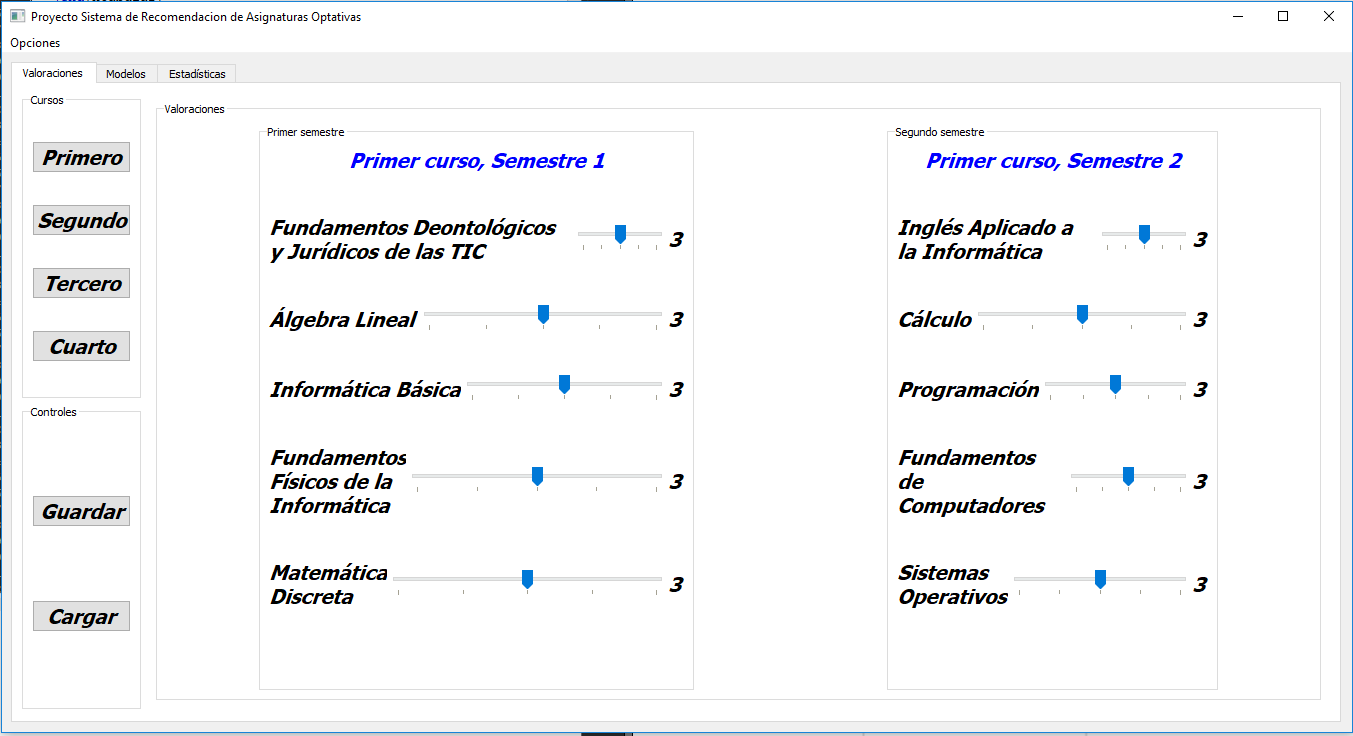
\includegraphics[width=0.90\textwidth]{INTERFAZ_Rellenado_Datos_V1-0}
\caption{Interfaz de rellenado de cuestionario}
\label{fig:E.2.1}
\end{figure}
Los cursos, son botones clicables, los cuales, al ser pulsados, muestran las asignaturas correspondientes a dicho año. \ref{fig:E.2.2}
\begin{figure}[h]
\centering
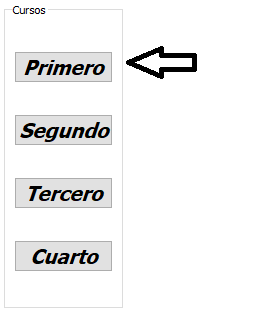
\includegraphics[width=0.90\textwidth]{cursos}
\caption{Cursos}
\label{fig:E.2.2}
\end{figure}

En caso de haberse registrado por primera vez, en el área central de la pantalla, las asignaturas constarán de valores medios, que deberán ser modificados por el usuario. \ref{fig:E.2.3}
\begin{figure}[h]
\centering
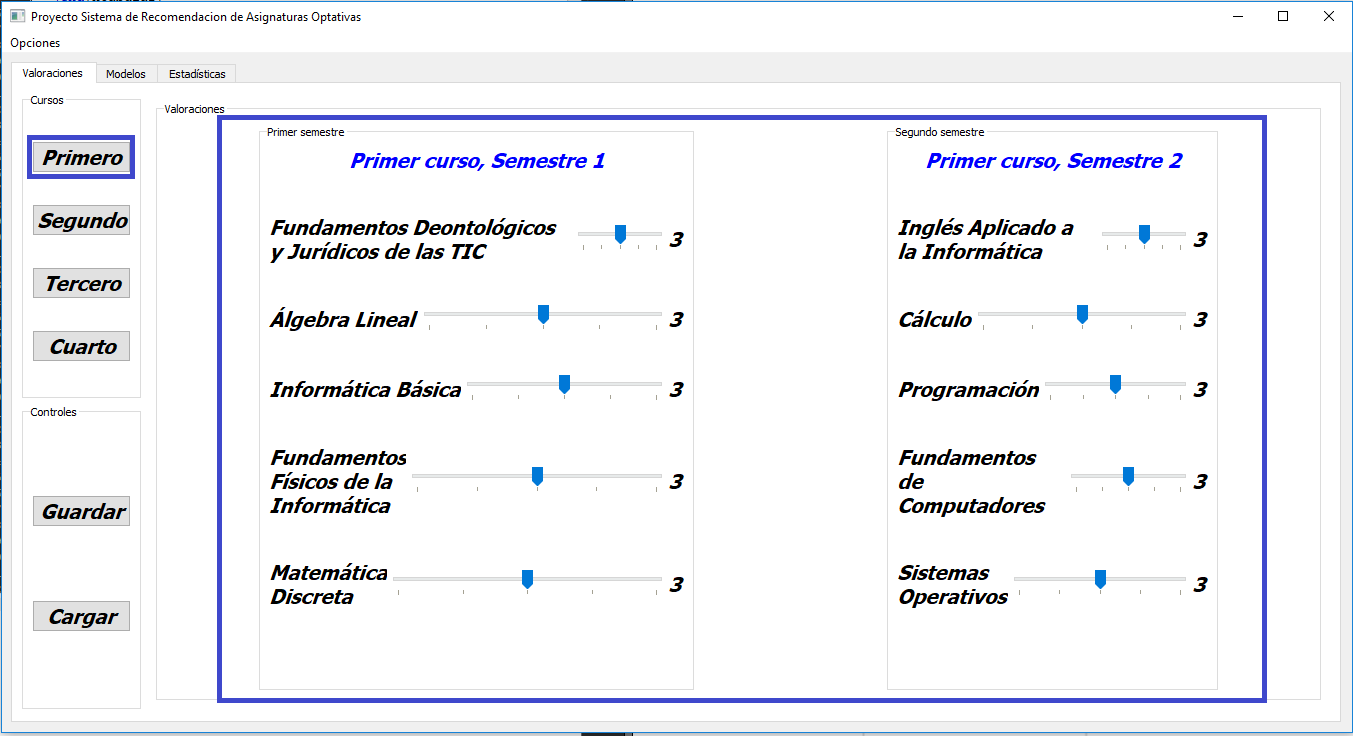
\includegraphics[width=0.90\textwidth]{INTERFAZ_Rellenado_Datos_Central_V1-0}
\caption{Parte central pestaña rellenado de datos}
\label{fig:E.2.3}
\end{figure}
Se pueden modificar las ponderaciones de las asignaturas bien con el ratón, arrastrando  slider, o bien con el teclado con las flechas izquierda y derecha. En la siguiente imagen se puede observar la diferencia entre utilizar el ratón y el teclado. \ref{fig:E.2.4}
\begin{figure}[h]
\centering
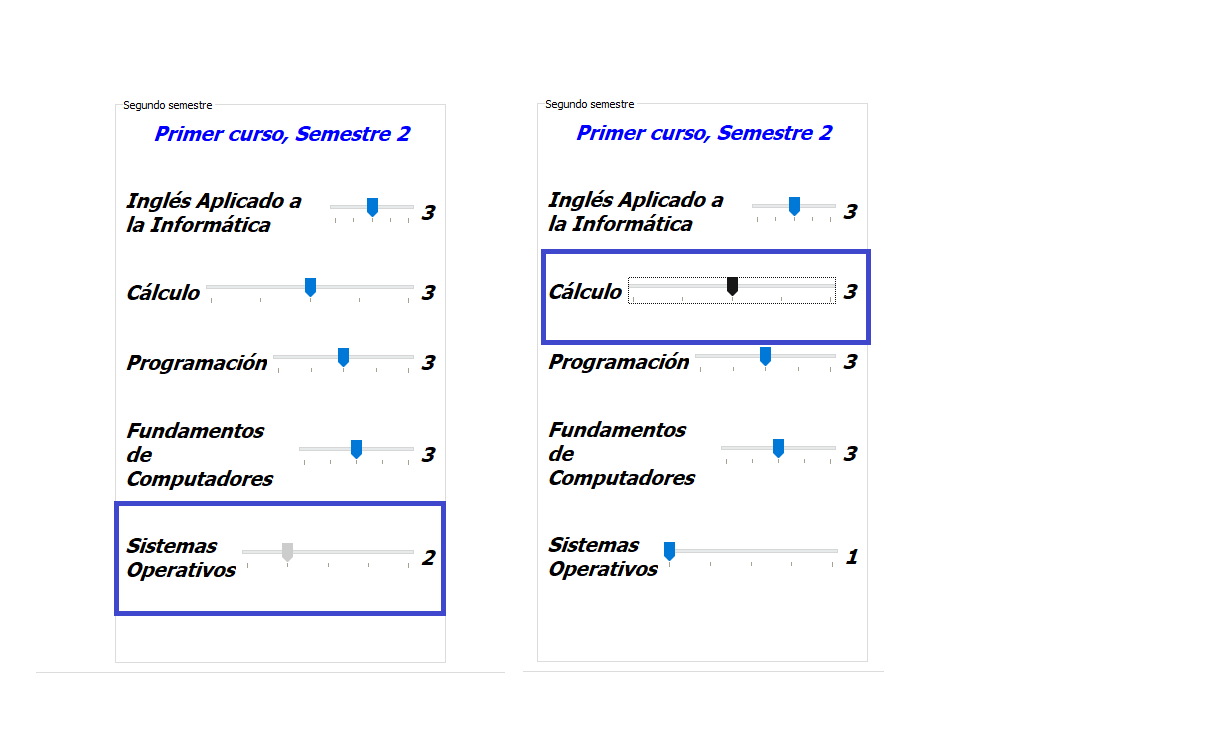
\includegraphics[width=0.90\textwidth]{INTERFAZ_Rellenado_Datos_Raton_V1-0}
\caption{Img Izq: Selección con ratón. Img Der: Selección con teclado}
\label{fig:E.2.4}
\end{figure}

En los botones de control, se permite \textbf{guardar} y \textbf{cargar} los datos. Al pulsar el botón guardar, se guardarán los datos introducidos de los cursos en un fichero binario, mientras que si se pulsa cargar, dichos datos se cargarán de forma automática. \ref{fig:E.2.5}
\begin{figure}[h]
\centering
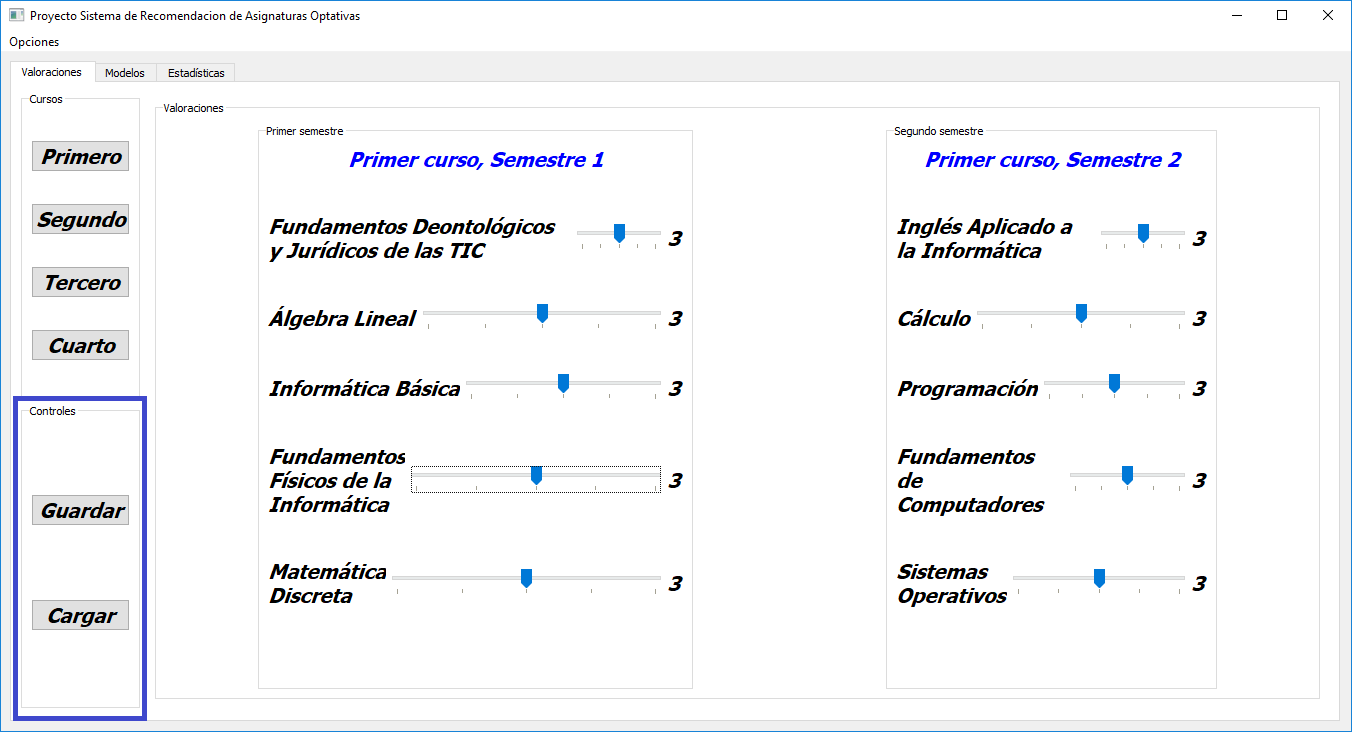
\includegraphics[width=0.90\textwidth]{INTERFAZ_Guarda_Carga}
\caption{Carga y guardado de datos}
\label{fig:E.2.5}
\end{figure}


\subsubsection{Version1.1}
La versión que será entregada de forma definitiva, y que será entregada al tribunal varía levemente en la interfaz gráfica. Al igual que en la Versión 1.0, aparece dicha ventana tras iniciar sesión. La ventana para la ponderación de las asignaturas tiene el siguiente aspecto: \ref{fig:E.2.5.1}
\begin{figure}[h]
\centering
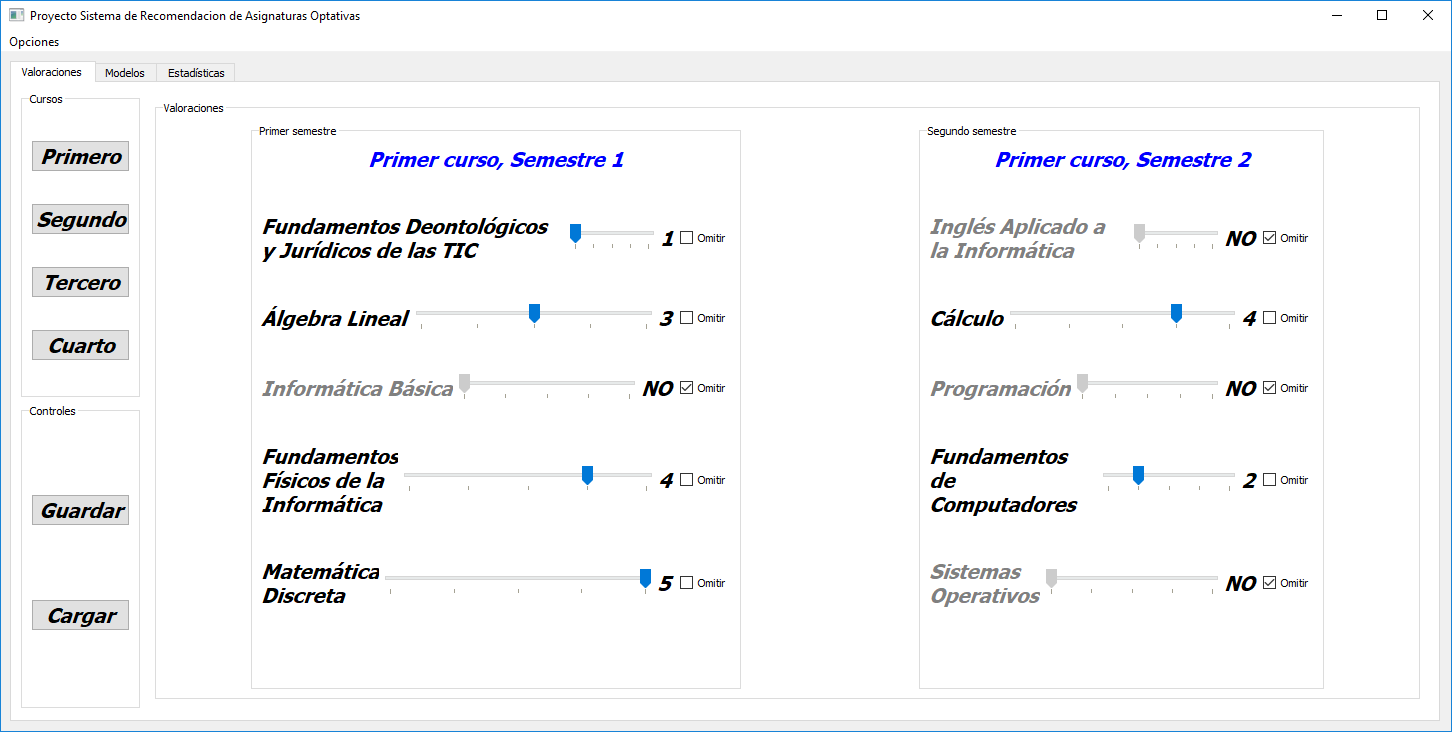
\includegraphics[width=0.90\textwidth]{INTERFAZ_1_1_Principal}
\caption{Pestaña principal versión 1.1}
\label{fig:E.2.5.1}
\end{figure}
\\Ahí radica la diferencia, en la posibilidad de no aplicar una asignatura determinada. Este cambio se debe a que hay alumnos que han convalidado ciertas asignaturas y no las han cursado en el Grado de Ingeniería Informática.\ref{fig:E.2.5.2}
\begin{figure}[h]
\centering
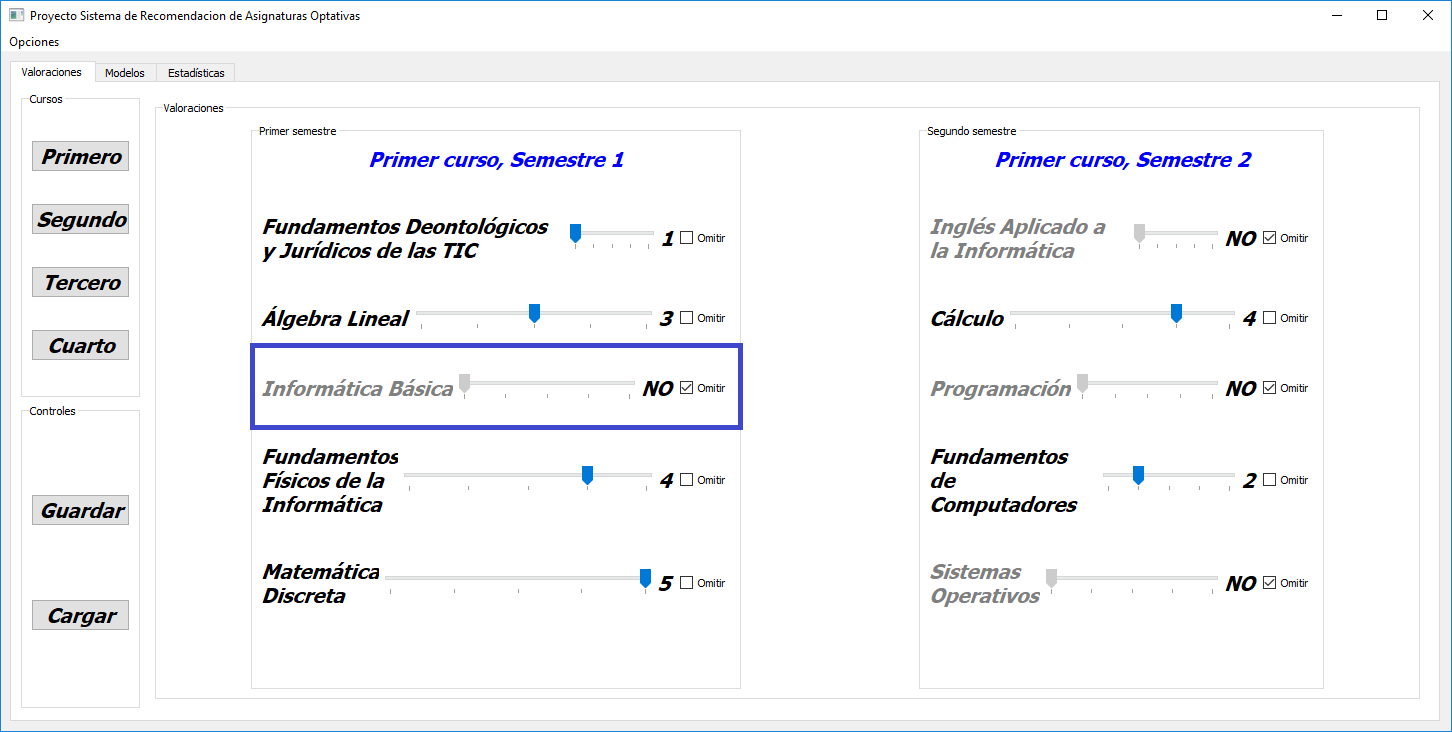
\includegraphics[width=0.90\textwidth]{INTERFAZ_1_1_Diferencia}
\caption{Diferencia respecto a la  versión 1.0}
\label{fig:E.2.5.2}
\end{figure} 
Exceptuando dicho cambio, el resto de las funcionalidades permanecen invariables. 

\subsection{Segunda pestaña}
La segunda pestaña, con las recomendaciones obtenidas, tienen el siguiente aspecto \ref{fig:E.2.6}
\begin{figure}[h]
\centering
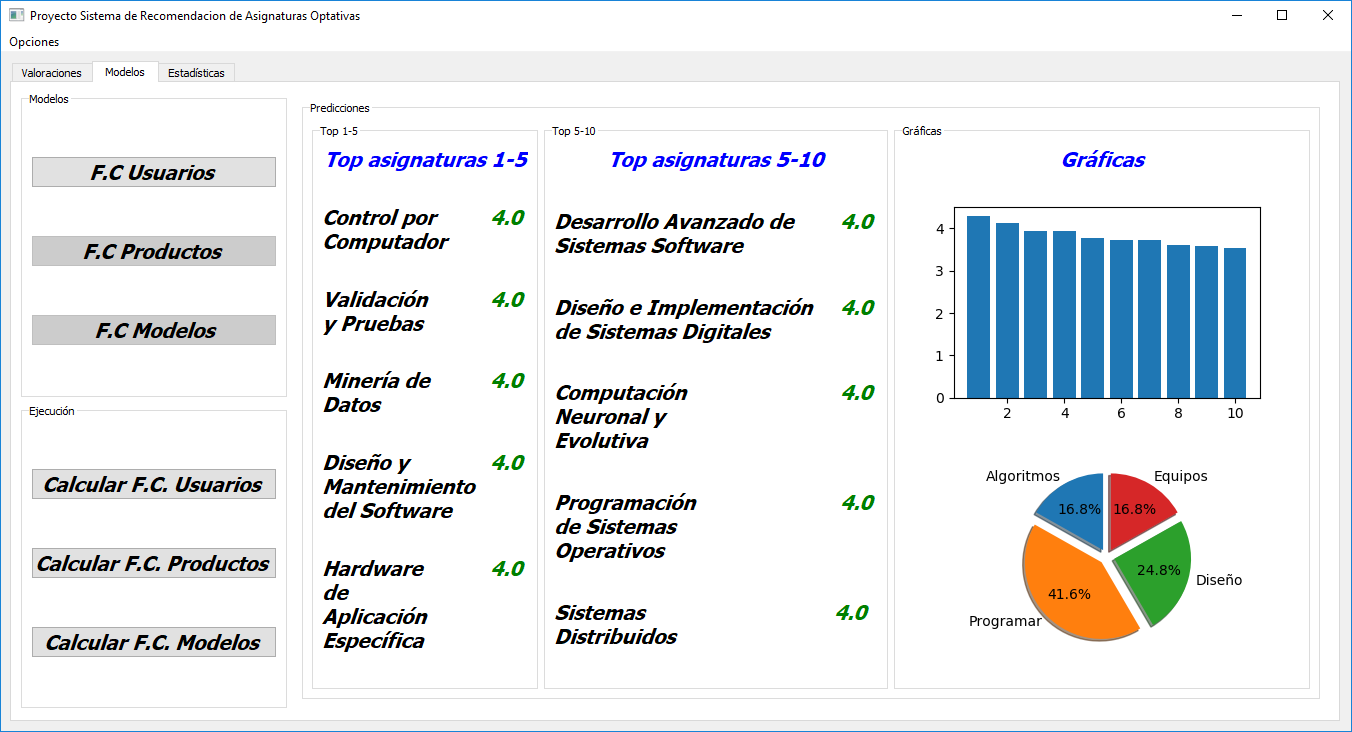
\includegraphics[width=0.90\textwidth]{INTERFAZ_Recomendacion_V1-0}
\caption{Recomendación por defecto}
\label{fig:E.2.6}
\end{figure}
La funcionalidad de dicha pestaña se puede subdividir en: 
\subsubsection{Selección y carga del sistema de recomendación}
El área izquierda se utiliza para seleccionar el sistema de recomendación, siendo por defecto el F.C basado en memoria basado en Usuarios, estando deshabilitados los demás filtros colaborativos. \ref{fig:E.2.7} \\Como se puede observar, únicamente el primer filtro se encuentra habilitado, mientras que los dos sucesivos (basado en productos y  Filtro Colaborativo basado en modelo) se encuentran deshabilitados. 
\begin{figure}[h]
\centering
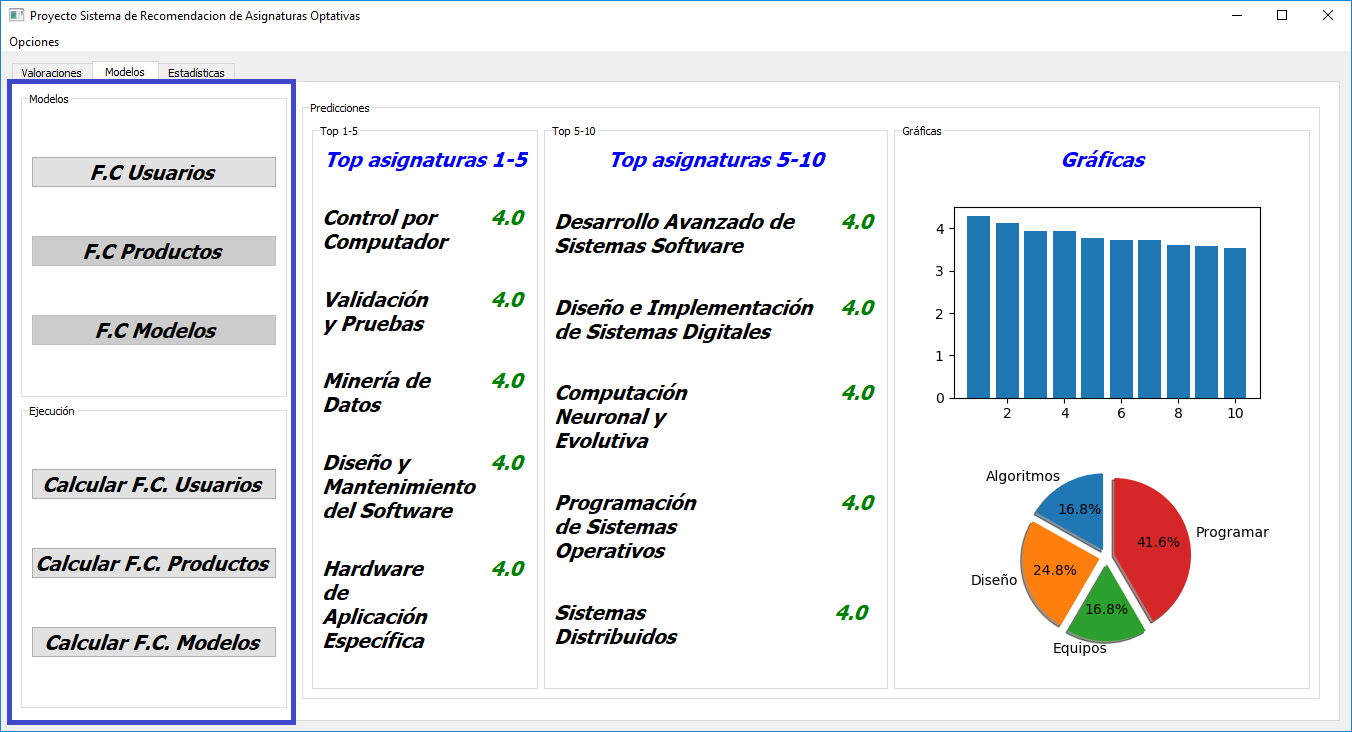
\includegraphics[width=0.90\textwidth]{INTERFAZ_seleccion_V1-0}
\caption{Muestra de los botones deshabilitados}
\label{fig:E.2.7}
\end{figure}
En cambio, si pulsamos el botón "Cargar F.C Productos" se habilita automáticamente la muestra de datos del Filtro Colaborativo basado en Productos. Esto lo podemos observar en la siguiente imagen, \ref{fig:E.2.8} en donde se ha pulsado el botón para el ejemplo. 
\begin{figure}[h]
\centering
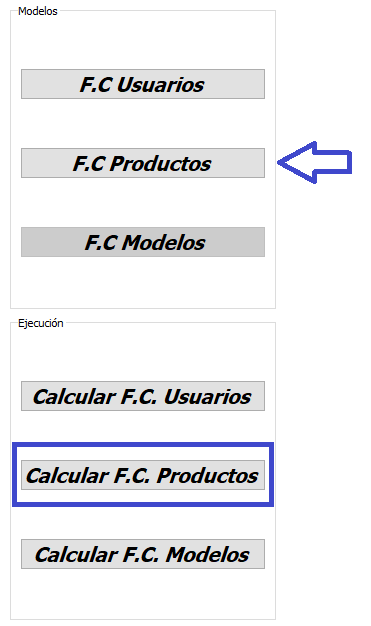
\includegraphics[width=0.90\textwidth]{INTERFAZ_seleccion2_V1-0}
\caption{Muestra de los botones habilitados tras pulsar cargar}
\label{fig:E.2.8}
\end{figure}
\\
Por otro lado, el área central indica las calificaciones redondeadas de las asignaturas recomendadas, con valores del 1-5, ordenadas de forma descendente.\ref{fig:E.2.9} 
\begin{figure}[h]
\centering
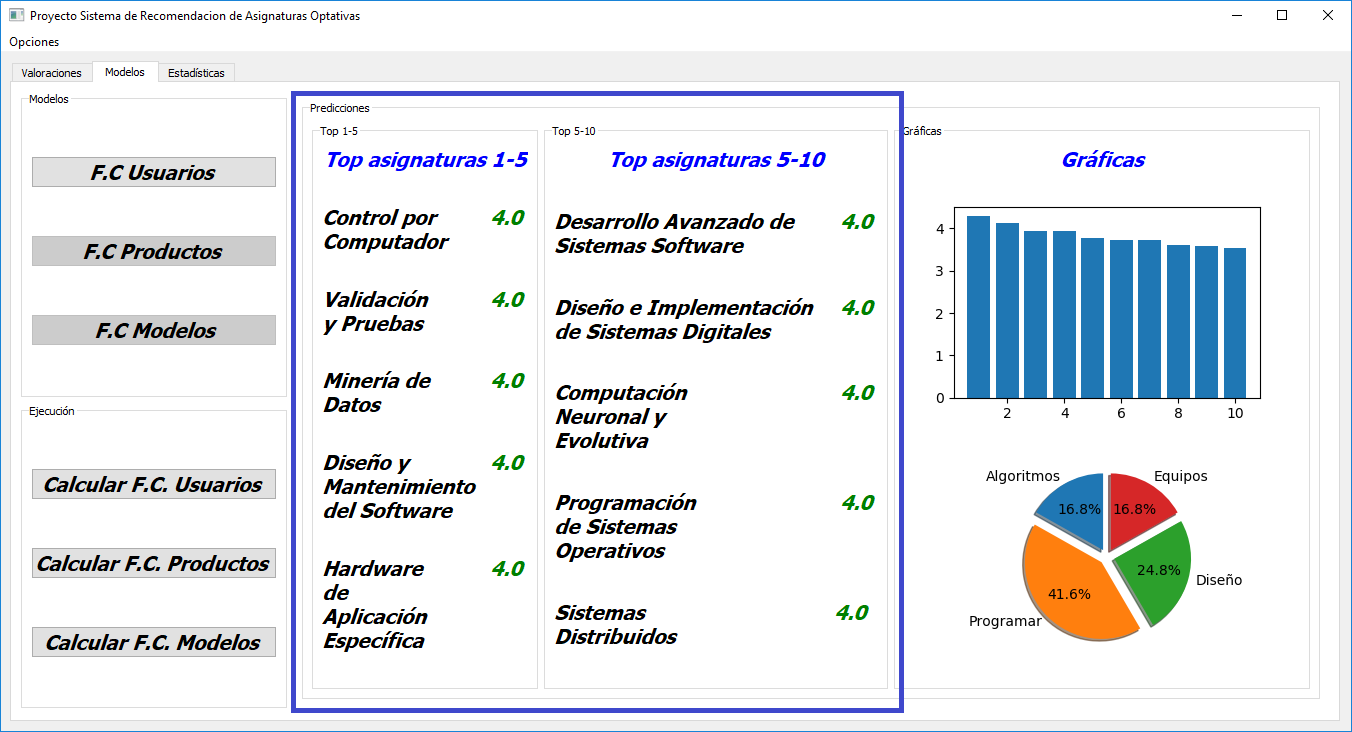
\includegraphics[width=0.90\textwidth]{INTERFAZ_Recomendacion_Asignaturas_V1-0}
\caption{Muestra de los resultados de un filtro colaborativo}
\label{fig:E.2.9}
\end{figure}
Para poder observar los valores reales que nos ha ofrecido el sistema de recomendación, deberíamos observar la gráfica de la derecha, en donde las calificaciones no están redondeadas. Para diferenciarlas, basta con colocar el ratón sobre una asignatura para observar el número de la asignatura, y poder verlo en la gráfica. \ref{fig:E.2.10} 
\begin{figure}[h]
\centering
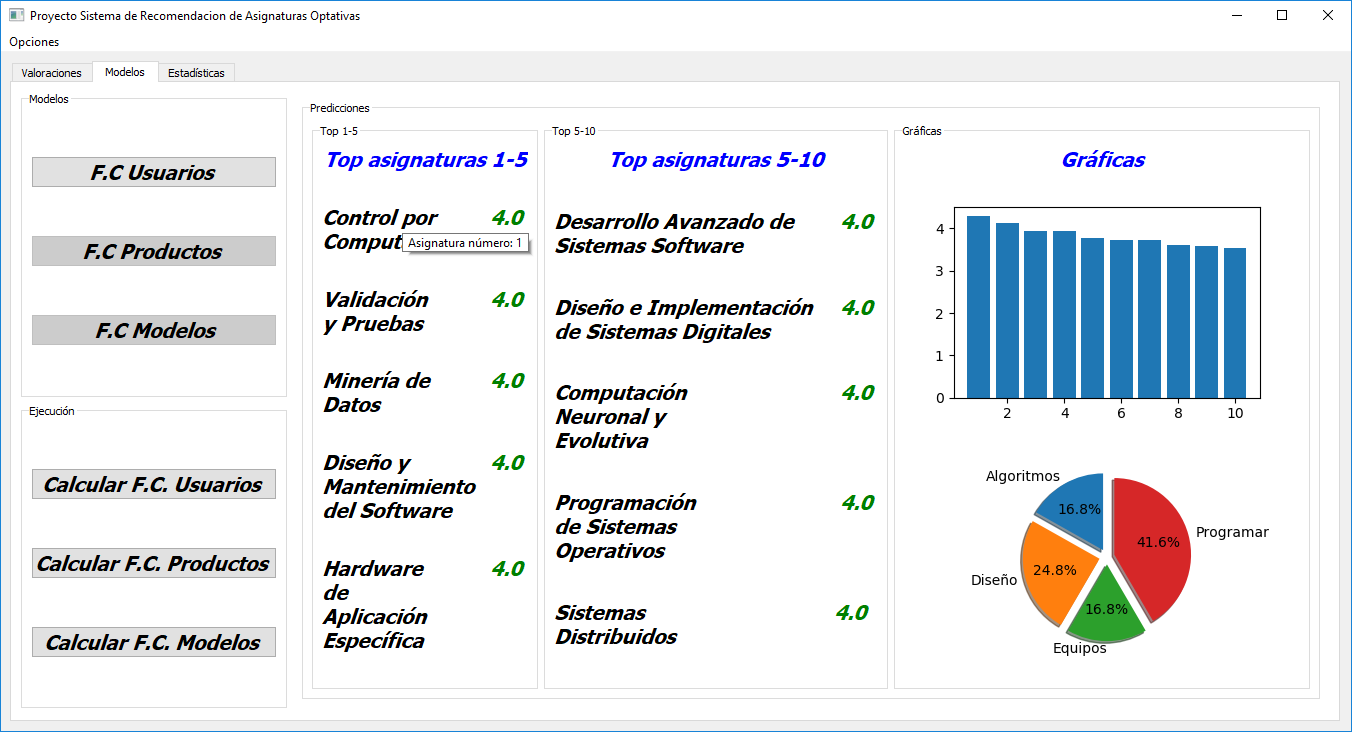
\includegraphics[width=0.90\textwidth]{INTERFAZ_Rellenado_Valores_V1-0}
\caption{Muestra del orden de la asignatura en la gráfica}
\label{fig:E.2.10}
\end{figure}
Así, podemos ver que, "Control por Computador", es la asignatura 1, por lo que en la gráfica, será la primera barra, con una ponderación ligeramente superior al 4. De esta forma, se puede observar que no todas las asignaturas tienen una calificación de 4, por lo que la gráfica de barras resulta útil para ver las diferencias entre las asignaturas. \ref{fig:E.2.11} 
\begin{figure}[h]
\centering
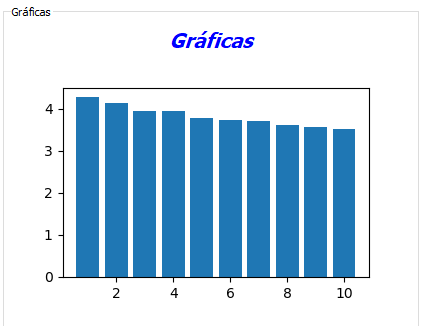
\includegraphics[width=0.90\textwidth]{INTERFAZ_Grafica_V1-0}
\caption{Muestra de la gráfica de asignaturas recomendadas}
\label{fig:E.2.11}
\end{figure}
\\Por otra parte, también tenemos un gráfico que indica las preferencias en los diferentes áreas del usuario, para indicar qué campos son de mayor interés para el mismo, de forma que el usuario pueda conocer el campo por el que se podría decantar en un futuro. \ref{fig:E.2.12} 
\begin{figure}[h]
\centering
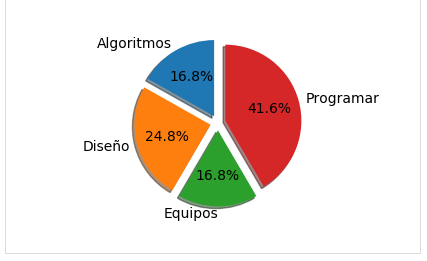
\includegraphics[width=0.90\textwidth]{INTERFAZ_Areas_V1-0}
\caption{Muestra de la gráfica de campos preferentes}
\label{fig:E.2.12}
\end{figure}
\\
Se debe tener en cuenta que dos sistemas de recomendación pueden ofrecer dos resultados diferentes para una misma asignatura, por lo que dichos resultados son meramente informativos. 

\subsection{Tercera pestaña}
La tercera pestaña contiene las medias, medianas, máximos y mínimos de las calificaciones insertadas por los usuarios de forma previa. De esta manera, se puede ver las relaciones de lo que ha seleccionado el usuario y las preferencias del resto de los usuarios. 
\\Las asignaturas se dividen en cursos, de forma que se puede ver las gráficas por cursos, siguiendo el patrón de la primera pestaña. 
\\La estructura de la pestaña tiene el siguiente aspecto: \ref{fig:E.2.13} 
\begin{figure}[h]
\centering
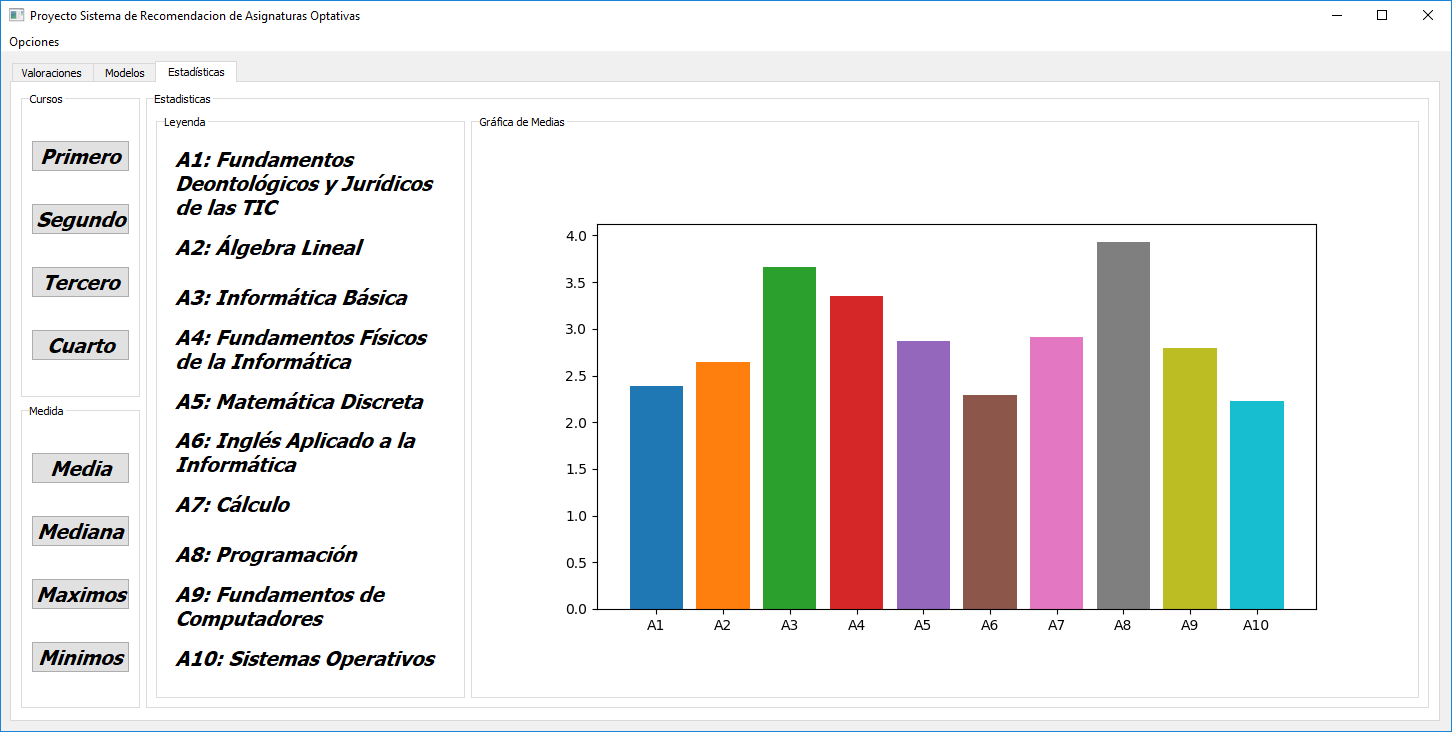
\includegraphics[width=0.90\textwidth]{INTERFAZ_Estadistica}
\caption{Muestra de la pestaña de estadísticas}
\label{fig:E.2.13}
\end{figure}
\\\\Al pulsar los diferentes cursos, obtenemos las pestañas, en donde en la leyenda indica el nombre de la asignatura y en la gráfica de barras su resultado. \ref{fig:E.2.14} 
\begin{figure}[h]
\centering
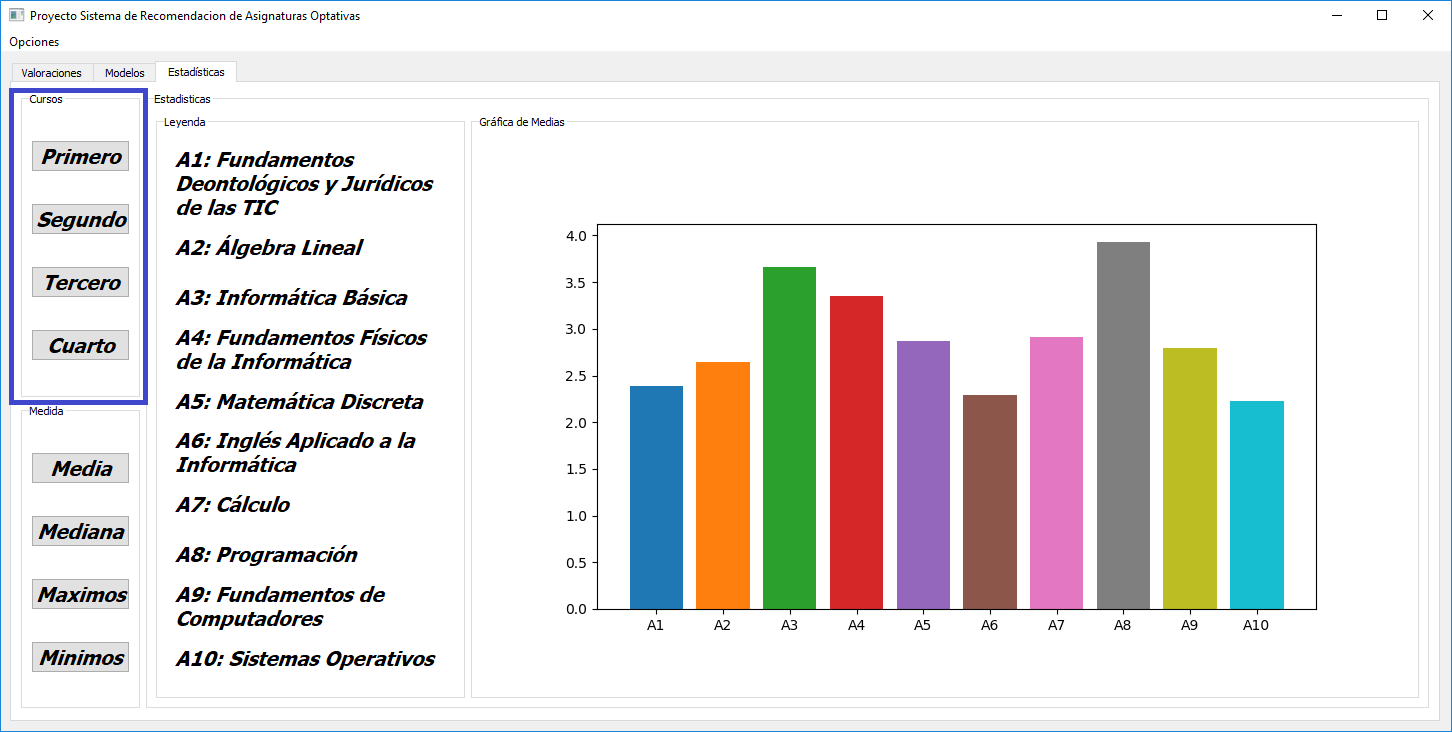
\includegraphics[width=0.90\textwidth]{INTERFAZ_Estadistica_cursos}
\caption{Muestra de los botones de la pestaña}
\label{fig:E.2.14}
\end{figure}
\\Tras seleccionar un curso deseado, automáticamente se calculan los valores de la modalidad en la que se esté (Medias, Medianas, Máximos y Mínimos), cambiándose automáticamente tanto la leyenda de las asignaturas como las ponderaciones. \ref{fig:E.2.15} 
\begin{figure}[h]
\centering
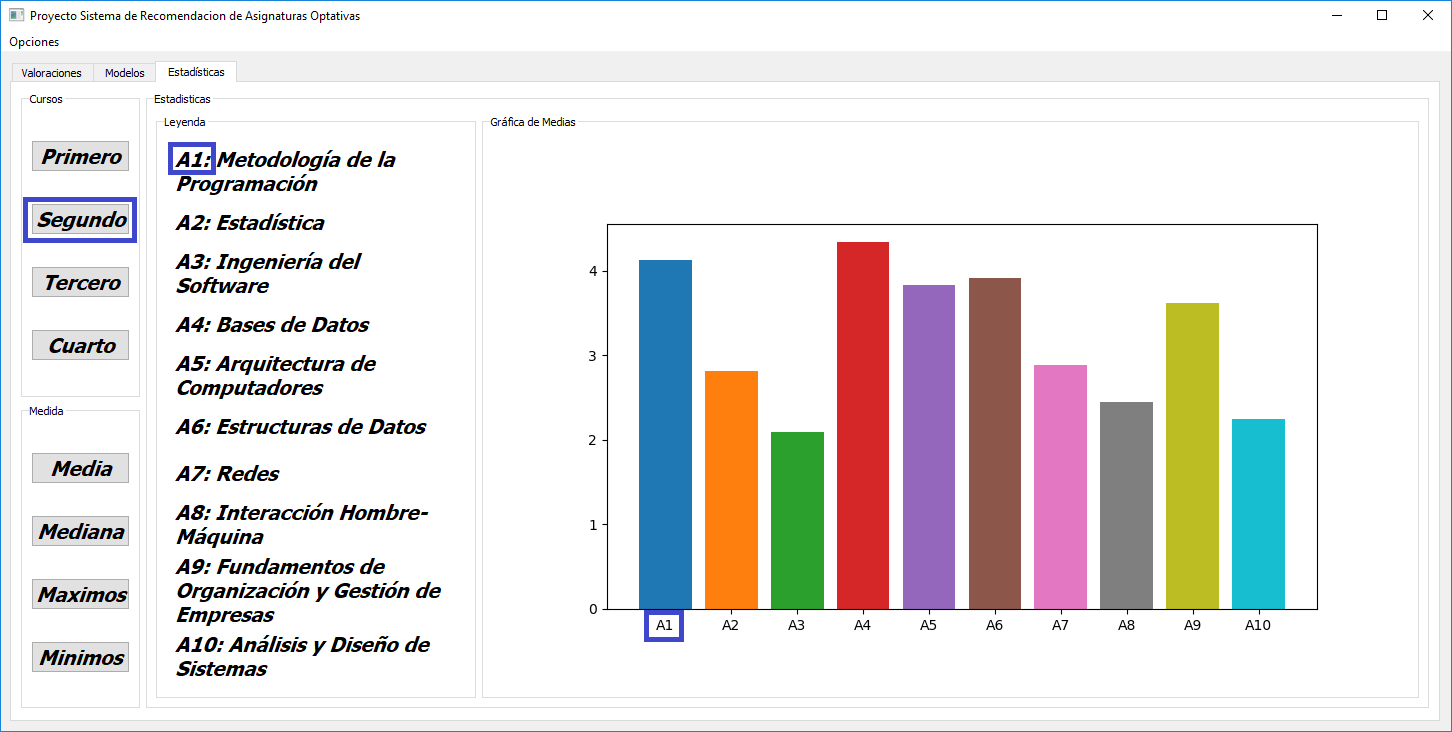
\includegraphics[width=0.90\textwidth]{INTERFAZ_Estadistica_media}
\caption{Ejemplo de media del segundo curso}
\label{fig:E.2.15}
\end{figure}
\\ De esta forma, podemos observar, que en el segundo curso, la asignatura A1 (Metodología de la Programación) tiene una media global de votaciones superior al cuatro. 
\\ Los máximos y mínimos corresponden con la calificación máxima y la mínima de las asignaturas entre los usuarios, de forma que, por ejemplo, para el cuarto curso, la calificación máxima de Diseño e Implementación de Sistemas Digitales es un 5 \ref{fig:E.2.16}, 
\begin{figure}[h]
\centering
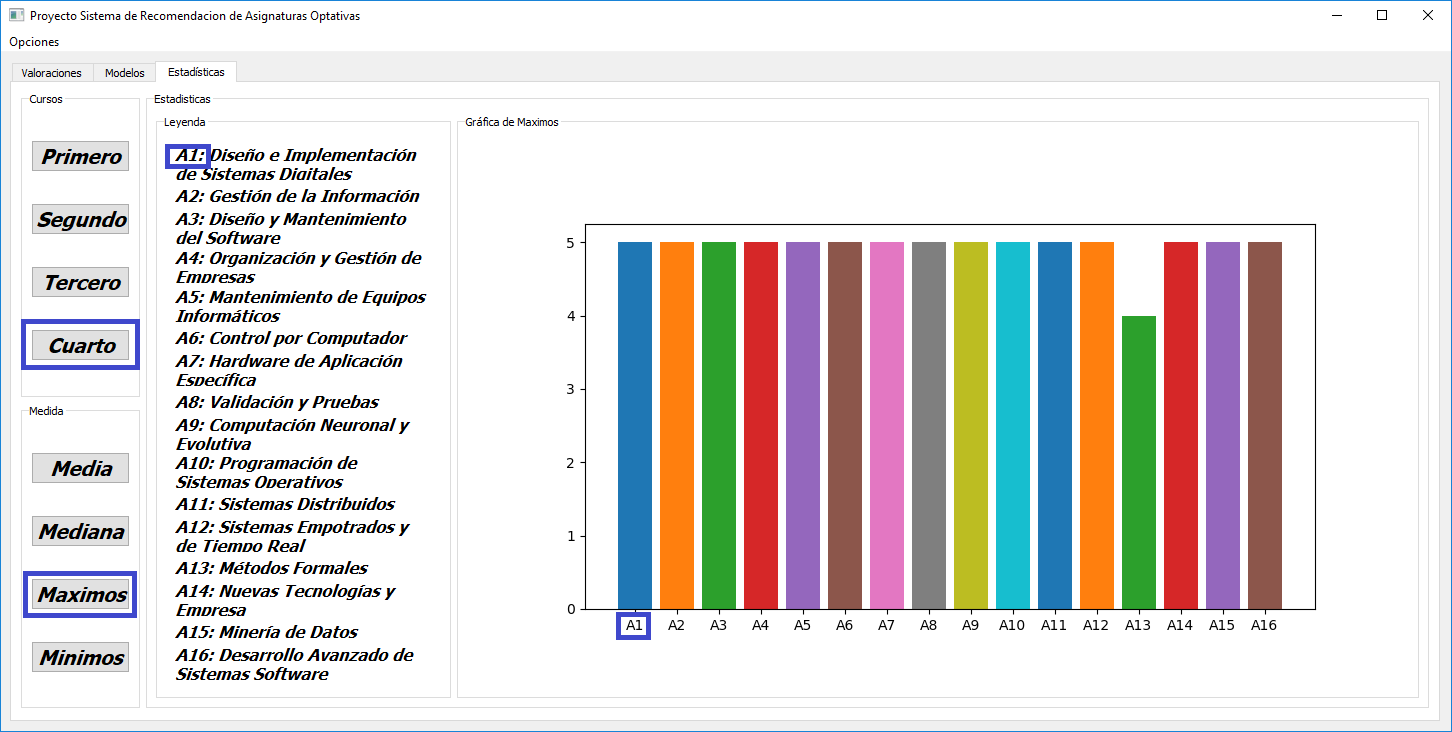
\includegraphics[width=0.90\textwidth]{INTERFAZ_Estadistica_maximos}
\caption{Ejemplo de máximos del cuarto curso}
\label{fig:E.2.16}
\end{figure}
mientras que el mínimo es un 1. \ref{fig:E.2.17}, 
\begin{figure}[h]
\centering
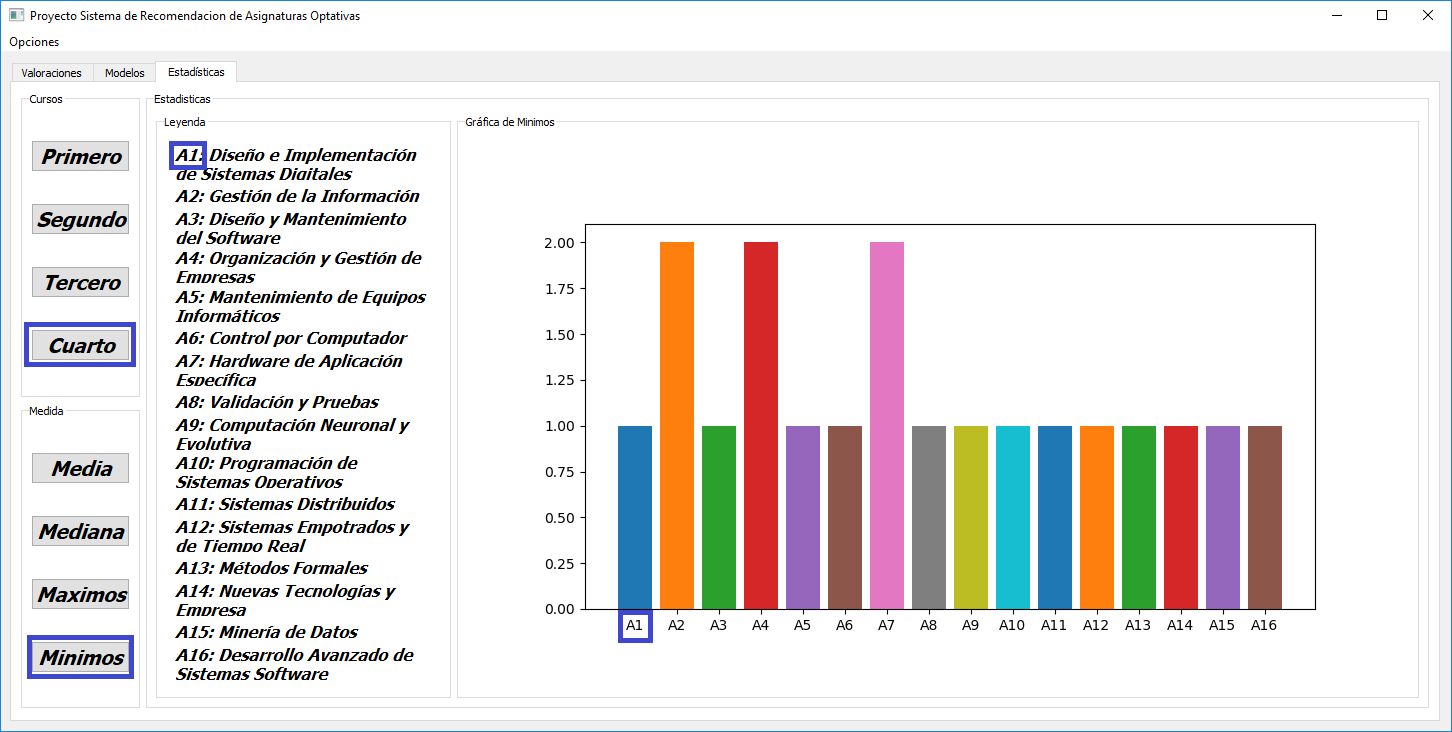
\includegraphics[width=0.90\textwidth]{INTERFAZ_Estadistica_minimos}
\caption{Ejemplo de mínimos del cuarto curso}
\label{fig:E.2.17}
\end{figure}









\bibliographystyle{plain}
\bibliography{bibliografiaAnexos}

\end{document}